\documentclass[11pt,letterpaper]{article}
\usepackage[T1]{fontenc}
\usepackage[utf8]{inputenc}
\usepackage{iftex}
\ifPDFTeX
\usepackage{mathptmx}
\else
\usepackage{fontspec}
\IfFontExistsTF{Times New Roman}{\setmainfont{Times New Roman}}{\setmainfont{TeX Gyre Termes}}
\fi
\usepackage[margin=1in]{geometry}
\usepackage{graphicx,longtable,array,setspace,multicol}
\usepackage[hidelinks]{hyperref}
\usepackage{caption}
\setlength{\parindent}{0pt}
\setlength{\parskip}{6pt}
\setlength{\emergencystretch}{3em}
\captionsetup{font=small,labelfont=bf}
\pagestyle{plain}
\begin{document}
\setlength{\parskip}{10pt}
\onehalfspacing
\pagenumbering{roman}
\begin{titlepage}\thispagestyle{plain}\centering\vspace*{1.2in}
{\LARGE\bfseries Stop Overthinking, Keep Passing the Tests\par}\bigskip
{\large Shortest Correct LoRA Training and Free Thinking Controls in Small Qwen3.5 Code Models\par}
\vspace{0.5in}A Thesis Submitted in Partial Fulfillment\\of the Requirements for the Degree of\\{}[DEGREE NAME] in [FIELD]\par
\vspace{0.4in}by\\{}[AUTHOR NAME]\\{}[STUDENT ID]\par
\vspace{0.5in}[DEPARTMENT]\\{}[UNIVERSITY]\\{}[CITY AND COUNTRY]\par\bigskip
[SUBMISSION MONTH AND YEAR]\end{titlepage}
\setcounter{page}{2}
\section*{Approval Page}
This thesis, titled ``Stop Overthinking, Keep Passing the Tests,'' was prepared by [AUTHOR NAME] and is submitted for review in partial fulfillment of the requirements for [DEGREE NAME] at [UNIVERSITY]. Approval and signatures are to be completed by the authorized committee.
\vspace{0.5in}\par\noindent\rule{2.8in}{0.4pt}\quad Date \rule{1in}{0.4pt}\par [SUPERVISOR NAME], Thesis Advisor
\vspace{0.5in}\par\noindent\rule{2.8in}{0.4pt}\quad Date \rule{1in}{0.4pt}\par [COMMITTEE MEMBER NAME], Committee Member
\vspace{0.5in}\par\noindent\rule{2.8in}{0.4pt}\quad Date \rule{1in}{0.4pt}\par [COMMITTEE MEMBER NAME], Committee Member
\clearpage\section*{Abstract}
Small language models can spend much of their output on explicit reasoning without producing correct code. We study whether shortest-correct low-rank adaptation training offers an advantage over simple thinking controls in Qwen3.5-0.8B, 2B, and 4B. The retrospective study combines saved outputs and grades for 464 unique problems: 164 HumanEval+ tasks and 300 LiveCodeBench tasks. Historical summaries average attempts within each problem and then give problems equal weight; completed-control comparisons separately use first attempts. All six LoRA-1 combinations with thinking OFF or a selected thinking limit are complete, with one answer per problem. LoRA plus OFF passes 65, 165, and 300 problems for the three sizes. LoRA plus limits of 512, 1,024, and 2,048 thinking tokens passes 67, 191, and 332 problems, corresponding to 14.4\%, 41.2\%, and 71.6\%. The 2B and 4B trained limits do not establish reliable accuracy gains over the matching free-limit first attempts. The 4B combination generates about 11.4\% fewer total output tokens than that reference. OFF without training remains the highest observed complete-set free score for 0.8B. Historical LoRA-2 and loop diagnostics retain their original 234-problem scope. The findings support testing strong free controls before investing in this training procedure. Conclusions remain limited by retrospective selection, historical environment differences, unadjusted intervals, one model family, and grading scope. Token reductions do not directly establish lower latency, cost, or energy use.
\par\bigskip\textbf{Keywords:} code generation; efficient reasoning; thinking budget; LoRA; Qwen3.5; benchmark evaluation.
\clearpage\section*{Acknowledgments}
We acknowledge the authors and maintainers of the models, datasets, evaluation tools, and open-source software used in this study. Their published resources make this work possible. Citations identify the research sources used in the thesis.
\par [PERSONAL ACKNOWLEDGMENTS: add verified names and any funding details before submission.]
\clearpage\tableofcontents
\clearpage\listoffigures
\clearpage\listoftables
\clearpage\section*{List of Abbreviations}
\begin{tabular}{ll}B & Billion parameters\\ CI & Confidence interval\\ CoT & Chain of thought\\ GPU & Graphics processing unit\\ LCB & LiveCodeBench\\ LLM & Large language model\\ LoRA & Low-rank adaptation\\ MBPP+ & MBPP with extended tests\\ OFF / ON & Explicit thinking disabled / enabled\\ PEFT & Parameter-efficient fine-tuning\\ pp & Percentage points\\ SFT & Supervised fine-tuning\end{tabular}
\clearpage\pagenumbering{arabic}


\section*{Chapter 1: Introduction}\addcontentsline{toc}{section}{Chapter 1: Introduction}

\subsection*{1.1 Background and Motivation}\addcontentsline{toc}{subsection}{1.1 Background and Motivation}

Language models can produce programs from a written problem statement. Some models first generate a reasoning trace, which is a sequence of notes before the final answer. These notes can help the model work through a difficult problem. They can also become long, repeat the same plan, or consume the space needed for the program. This thesis asks how much of that written reasoning is useful for small code-generating models. It studies an operational question: should a user train a small model to reason more briefly, or first try the thinking controls already available in the model?\par

The title, Stop Overthinking, Keep Passing the Tests, describes the desired behavior. A useful system should produce correct code without unnecessary output. However, the title is a research goal rather than a promise that every experiment achieves both aims. The evidence shows a more careful pattern. Different model sizes benefit from different controls, and an improvement over unrestricted thinking does not automatically show that training was necessary. A trained model must also be compared with an untrained model using the same thinking setting.\par

Research on efficient reasoning considers ways to control the amount of work a model expresses before answering \cite{survey}. This study focuses on three Qwen3.5 sizes: 0.8B, 2B, and 4B, where B refers approximately to billions of parameters \cite{q08,q2,q4}. Small models are a useful setting because they offer a practical route to experiments on a single accelerator. Nevertheless, a model being small does not make its output automatically short or reliable. Output behavior still needs direct measurement.\par

We compare thinking ON, thinking OFF, fixed thinking limits, and trained low-rank adaptation add-ons. Low-rank adaptation, abbreviated LoRA, changes a small set of trainable matrices while retaining the base weights \cite{lora}. The training idea is to generate several solutions to practice problems, retain short solutions that pass tests, and train an add-on on these examples. Self-training with concise solutions provides the motivation for this approach \cite{selftrain}. The thesis tests this idea in the repository's specific code setting; it does not assume that findings from another task transfer unchanged.\par

Correctness is checked through saved benchmark grades. An answer must pass the tests actually used by the grader. This is more concrete than judging whether an explanation sounds convincing. It is also narrower than proving that a program works on every possible input. The distinction matters because a program can pass a limited collection of tests and still contain an error. Accordingly, this thesis uses the term observed accuracy for the measured result and states the testing scope alongside it.\par

The practical motivation is a limited experimental budget. Before collecting many training examples, a researcher can switch thinking off or set a thinking-token budget. These controls require no additional training, although generating answers still consumes computing resources. We call them free controls only in that restricted sense. Whether an intervention saves time, energy, or money requires separate measurements. Here, output length is measured in tokens and is treated as a resource proxy rather than a direct bill.\par

\begin{center}\begin{minipage}{\linewidth}\centering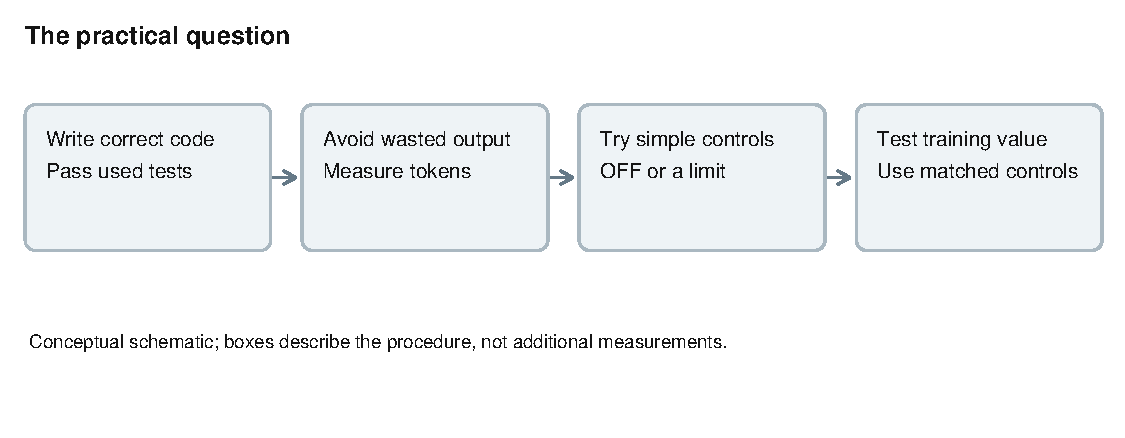
\includegraphics[width=\linewidth]{figures/motivation.pdf}\captionof{figure}{The practical decision joins correctness and generated length. This is an explanatory diagram, not a new experiment.}\label{fig:motivation}\end{minipage}\end{center}

\subsection*{1.2 Problem Statement}\addcontentsline{toc}{subsection}{1.2 Problem Statement}

The central problem is whether shortest-correct LoRA training provides a useful advantage over simple thinking controls for small Qwen3.5 code models. The desired advantage concerns correctness and output length together. A method that writes fewer tokens but fails more problems may be unsuitable. A method that passes slightly more problems while adding training work may also be difficult to justify if a matched free control achieves a similar result.\par

There are two distinct comparisons. The first asks whether training alone improves on the base model with unrestricted thinking. The second asks whether the same trained add-on helps after thinking is switched off or limited. These questions cannot be answered by comparing a trained limited model only with an unrestricted base model. Such a comparison changes both training and inference policy at once. We therefore identify the matching untrained policy whenever interpreting an apparent training benefit.\par

The evidence comes from saved experiments collected in stages. It is not a newly randomized, single-session evaluation. The combined test set contains 464 unique problems, but older configurations can have more attempts on some problems than on others. Some exploratory methods cover only a subset. A central methodological requirement is to preserve those differences rather than make a large table that hides them. Equal weighting by problem and separately labeled first-attempt comparisons are used for that purpose.\par

\subsection*{1.3 Research Questions and Objectives}\addcontentsline{toc}{subsection}{1.3 Research Questions and Objectives}

RQ1 asks how thinking ON, thinking OFF, and the selected full-coverage thinking limits compare in observed accuracy and output tokens for each model size. The objective is to establish useful untrained references before assessing an add-on. The comparison is restricted to measured settings and does not identify the best possible budget.\par

RQ2 asks whether LoRA-1 alone improves over the corresponding untrained controls. The objective is to separate the effect of learned concise examples from the effect of an inference-time switch. LoRA-1 alone always means that thinking is ON without an additional thinking-token limit.\par

RQ3 asks whether LoRA-1 combined with OFF or a selected limit improves over the same setting without LoRA. The objective is to evaluate all six completed combinations: two controls for each of three model sizes. Each combination has one saved answer on each of the same 464 problems.\par

RQ4 asks how the results vary between HumanEval+, LiveCodeBench easy, and LiveCodeBench medium problems. The objective is to show whether a combined score conceals a major difference between short function tasks and contest-style tasks. HumanEval+ is presented as its own benchmark group rather than treated as directly equivalent to a contest difficulty label.\par

RQ5 asks what the historical training and repetition evidence can explain, and where it stops. The objective is to distinguish observed associations from causal explanations. Earlier LoRA-2 and loop analyses retain their original 234-problem scope and are not generalized into measurements on the full combined set.\par

\subsection*{1.4 Scope and Limitations}\addcontentsline{toc}{subsection}{1.4 Scope and Limitations}

The main study includes 164 HumanEval+ problems and 300 LiveCodeBench problems, comprising 166 easy and 134 medium contest tasks. There are no hard LiveCodeBench tasks in the combined set. The work evaluates Python code generation in one model family. It does not establish performance for mathematics, open-ended question answering, repository-level software maintenance, or other programming languages.\par

The outcome is based on existing grades. HumanEval+ uses extended tests, while the saved LiveCodeBench evaluation uses up to 20 tests per problem. A pass therefore means that the extracted code passed those used tests. The document rebuild neither executes the generated code again nor changes a grade. This keeps the report tied to the historical measurements and avoids silently creating a different evaluation.\par

The combined view was chosen after results were available. Some historical controls were run under different package versions or batch layouts from the completed combinations. A matching random seed does not remove every environmental difference. These are limitations of causal interpretation, not reasons to discard the measurements. The correct response is to state the comparison and its provenance clearly.\par

We do not measure human preference for explanations, source-code maintainability, wall-clock inference latency across all configurations, energy consumption, or deployment cost. Token reductions are reported directly. They are not converted into unsupported claims about money or environmental impact. Likewise, the absence of exact training/test ID overlap does not prove that the base model never encountered similar tasks during pretraining.\par

\subsection*{1.5 Contributions}\addcontentsline{toc}{subsection}{1.5 Contributions}

The first contribution is a unified account of a completed three-size study using 464 distinct test problems. The report connects model settings, coverage, accuracy, output length, and uncertainty. Its contribution is an empirical comparison with transparent boundaries, rather than a new base-model architecture.\par

The second contribution is the completed evaluation of all six LoRA-1 combinations with OFF and selected thinking limits. Using the same test IDs makes it possible to ask whether a trained add-on contributes beyond a simple inference policy. The result is useful even when the answer is inconclusive: it identifies which apparent gains are supported and which require a stronger follow-up experiment.\par

The third contribution is a reporting framework that keeps two summaries distinct. The historical combined view averages available attempts within each problem and then averages across problems. The completed-control view uses one attempt per problem and compares with historical first attempts. These views answer related but different questions. Presenting both prevents a rounded percentage from changing meaning between sections.\par

The fourth contribution is an evidence-based explanation for readers new to reasoning models. Diagrams separate training from inference, thinking tokens from total output tokens, and cap hits from detected repetition. Tables and figures are built from the saved result files, so the simplified explanation remains connected to the numerical record.\par

\subsection*{1.6 Thesis Organization}\addcontentsline{toc}{subsection}{1.6 Thesis Organization}

Chapter 2 explains the relevant concepts and places the study within efficient reasoning, self-training, LoRA, and code evaluation research. Chapter 3 describes the datasets, training procedure, generation settings, scoring rules, uncertainty calculations, and validation checks. Chapter 4 presents the complete and partial results with their actual coverage. Chapter 5 interprets the findings and discusses alternative explanations and practical implications. Chapter 6 answers the research questions and proposes specific follow-up experiments. References provide the cited sources, and the appendices document the result files, test IDs, and reproduction steps.\par

\clearpage

\section*{Chapter 2: Literature Review}\addcontentsline{toc}{section}{Chapter 2: Literature Review}

\subsection*{2.1 Language Models and Program Generation}\addcontentsline{toc}{subsection}{2.1 Language Models and Program Generation}

A language model generates a sequence by repeatedly predicting the next token. A token may be a word, part of a word, punctuation, or a piece of code. The relationship between tokens and words varies by text and tokenizer, so the token counts in this thesis are not converted into exact word counts. Parameters are the learned numbers that determine the model's predictions. The size labels 0.8B, 2B, and 4B describe approximate parameter scales, not the number of tokens used to answer a question.\par

For a coding task, the prompt describes the desired behavior and the model produces a function, class method, or complete program. This output has two kinds of requirements. It must be expressed in a form that the evaluation system can run, and it must implement the intended computation. A correct algorithm in an unusable response format can still fail evaluation. Conversely, a perfectly formatted program can produce the wrong answer. Studying generation therefore requires keeping task semantics and answer format in view.\par

The model does not inspect the future grader result when producing a normal test answer. Grading is a separate operation performed after generation. This separation is essential for interpreting the training pipeline: practice answers may be selected using their tests, but test answers cannot be selected by looking at their final grades and then called single-attempt performance. The present completed configurations each retain one answer per test problem.\par

\subsection*{2.2 Written Reasoning and Its Limits}\addcontentsline{toc}{subsection}{2.2 Written Reasoning and Its Limits}

In the study's generation format, thinking is the text before a designated boundary and the final answer follows that boundary. This is an observable output convention. It should not be taken as a complete description of every computation inside the model. Thinking OFF removes the explicit reasoning channel from the response policy; it does not mean that the neural network performs no computation.\par

Written reasoning can organize a solution, identify constraints, or check an algorithm. However, every additional note also consumes output space. If a model repeatedly restates its plan, fewer tokens may remain for executable code before the overall output cap is reached. A fixed thinking budget attempts to manage that allocation. It reserves the possibility of producing an answer by ending the notes, but it cannot guarantee that the notes contain a correct solution.\par

The efficient-reasoning survey by Sui and colleagues organizes a broad area concerned with reducing unnecessary reasoning work \cite{survey}. That literature motivates measuring resource use alongside answer quality. Our use of the term overthinking is narrower and operational: output may be longer than is useful under the tested conditions. We do not assign a hidden optimal reasoning length to every problem.\par

\begin{center}\begin{minipage}{\linewidth}\centering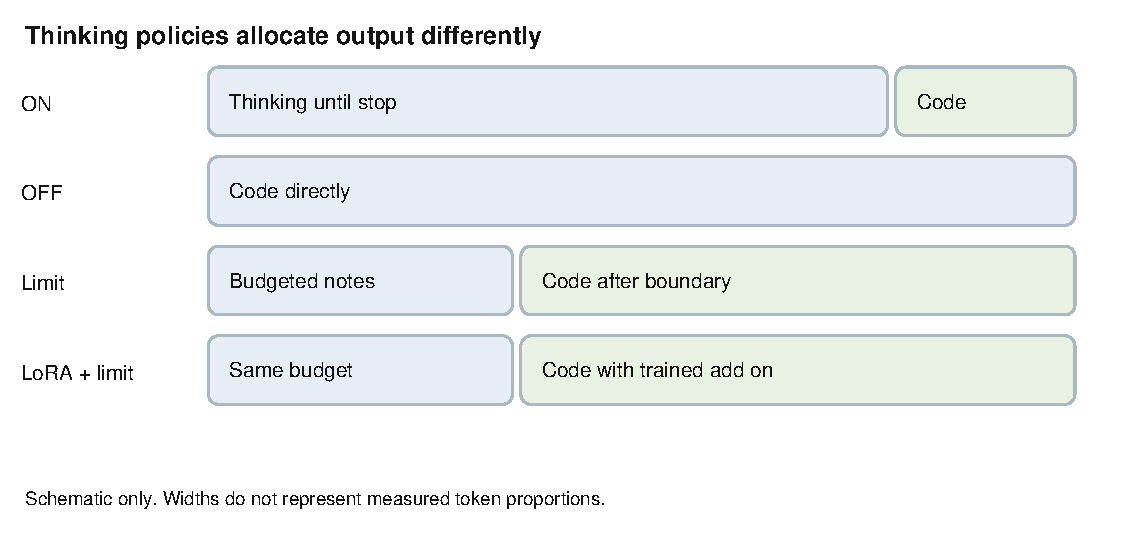
\includegraphics[width=\linewidth]{figures/controls.pdf}\captionof{figure}{ON, OFF, and limits differ in how explicit notes precede the answer. LoRA can be combined with these policies; widths are schematic.}\label{fig:controls}\end{minipage}\end{center}

\subsection*{2.3 Self Training with Concise Solutions}\addcontentsline{toc}{subsection}{2.3 Self Training with Concise Solutions}

Munkhbat and colleagues study self-training from concise model-generated reasoning paths \cite{selftrain}. Their method uses the model's own successful outputs as learning material. Their reported setting includes mathematics tasks and shows that concise self-generated supervision can reduce output while preserving average accuracy. This provides a motivation for shortest-correct selection, but it does not establish that the same selection rule will work on this thesis's small coding models.\par

The general idea is easy to explain. A student tries a practice question several times, checks which attempts work, and studies one of the shorter successful approaches. The model version generates multiple candidates, checks them, and uses selected examples as supervised training targets. This process differs from merely telling the model to be brief at test time. The former updates a trained add-on; the latter changes only the prompt.\par

Selection introduces its own bias. A practice problem with no passing candidate contributes no successful target. A problem with many correct candidates offers more opportunity to find a short one. Therefore, the retained examples describe problems the model could already solve under the sampling procedure. They are not a random sample of all difficult situations encountered at test time. This observation is a methodological implication of the selection process and is not an additional experimental finding.\par

The current study also uses a length guard in its historical selection pipeline. The intention is to avoid learning from unusually short answers that omit useful reasoning. A guard can limit extreme selection, but it cannot create concise successful answers when all successful candidates are long. The retained training distribution must therefore be examined, rather than described only by the number of starting problems.\par

\subsection*{2.4 Compression and Software Engineering Research}\addcontentsline{toc}{subsection}{2.4 Compression and Software Engineering Research}

SEER studies self-enhancing chain-of-thought compression for reasoning models in software engineering \cite{seer}. Its verified publication record describes best-of-N sampling, filtering, and fine-tuning on a DeepSeek-R1-Distill-Qwen-7B backbone. The reported average reasoning-length reduction is 34.6\% across its evaluated software engineering benchmarks. The relevant lesson is that successful compression is possible in an explicitly studied setting; its percentage is not a target or predicted outcome for Qwen3.5-0.8B, 2B, or 4B.\par

ASAP uses anchor-guided and surprisal-based pruning to identify parts of a reasoning trace for compression \cite{asap}. Its intervention differs from simply choosing the shortest correct whole answer. That difference matters when comparing methods: two systems may both produce shorter text while learning from very different supervision. This thesis evaluates the saved shortest-correct add-ons and does not implement ASAP's pruning procedure.\par

These approaches suggest several possible sources of transfer differences. A larger model may have a broader pool of correct candidate solutions. A pruning procedure may preserve a useful intermediate step that whole-answer length selection overlooks. A training dataset may resemble the test distribution more closely in one study than another. These are candidate explanations to investigate, not claims that this thesis has isolated their effects.\par

\subsection*{2.5 Low Rank Adaptation}\addcontentsline{toc}{subsection}{2.5 Low Rank Adaptation}

Hu and colleagues introduce LoRA as a way to adapt a pretrained model by learning low-rank updates while freezing the original weights \cite{lora}. The decomposition reduces the number of trainable parameters compared with updating every weight. In this study, the term add-on refers to the saved LoRA parameters used with the associated base checkpoint. It is an explanatory term for the reader, not a separate technical method.\par

For a weight matrix W, a simplified expression is W effective = W frozen + (alpha/r) BA. The matrices A and B form the learned update, r is the rank, and alpha controls its scale. This expression describes the adaptation idea. It does not imply that every implementation target, quantization choice, or inference kernel is identical across the historical runs. Those details belong in the saved adapter and environment records.\par

\begin{center}\begin{minipage}{\linewidth}\centering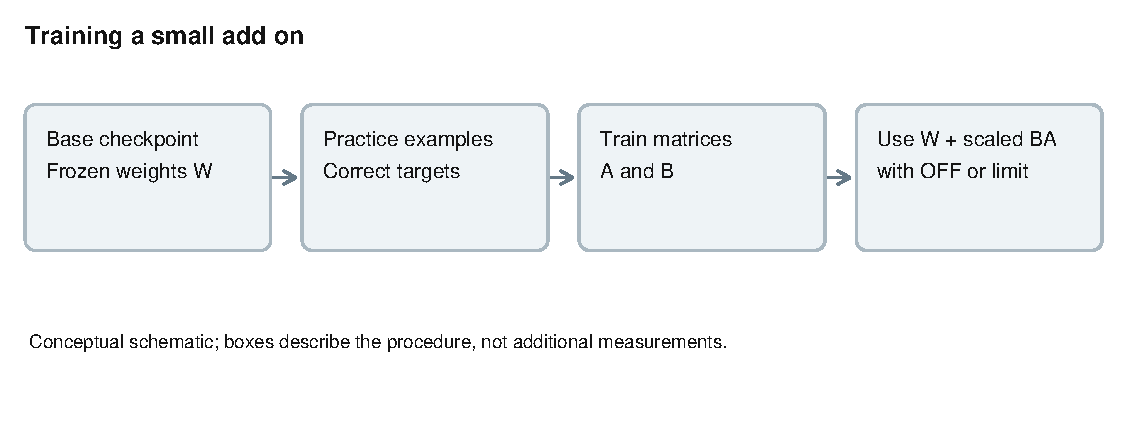
\includegraphics[width=\linewidth]{figures/lora.pdf}\captionof{figure}{Conceptual LoRA pipeline. Training and the later thinking policy are separate choices.}\label{fig:lora}\end{minipage}\end{center}

LoRA is an optimization mechanism, not a guarantee of improved reasoning. Its outcome depends on the base model, target examples, training settings, and test distribution. A training loss can fall because the add-on fits its examples even when the measured test behavior does not improve. Thus the thesis treats loss as evidence about training fit and uses held-out code grades to assess the task outcome.\par

There is also an important distinction between a training pool and a retained training set. A pool is the collection of problems used to generate candidates. The retained set contains the selected examples that actually enter training. Stating only the pool size can overstate how much successful supervision was available. Chapter 3 reports both where they are supported by the saved records.\par

\subsection*{2.6 Thinking OFF and Budget Controls}\addcontentsline{toc}{subsection}{2.6 Thinking OFF and Budget Controls}

Ma and colleagues show that bypassing explicit thinking can be a competitive strategy under constrained budgets \cite{nothink}. Their study includes coding among several task types. It establishes a reason to take OFF seriously as a baseline, rather than assuming that any reasoning trace must help. The present work uses its own model controls and single-answer outcomes; it does not reproduce that paper's parallel sampling or aggregation results.\par

The s1 work studies test-time scaling and includes budget forcing that can terminate or extend a model's reasoning \cite{s1}. For this thesis, the relevant concept is the ability to intervene on the amount of explicit reasoning before the answer. The tested fixed limits are an inference control. They do not require retraining a model each time the budget changes.\par

The official Qwen3.5 model cards document the model family and thinking-related usage \cite{q08,q2,q4}. Those cards establish the identity and supported interfaces of the checkpoints. They do not replace the experiment's actual configuration files. A thesis must report what the saved runs used, even if a later recommended library version or default setting differs.\par

The controls in this study are not interchangeable. OFF requests direct answering. A limit permits a bounded amount of notes. A brief prompt asks the model to regulate its own response. A model can obey one control and respond poorly to another. Consequently, this thesis reports a prompt-specific historical failure as a result for that wording, not a proof that every concise prompt is ineffective.\par

\subsection*{2.7 Benchmarks and Functional Correctness}\addcontentsline{toc}{subsection}{2.7 Benchmarks and Functional Correctness}

EvalPlus strengthens code evaluation by adding test cases to existing benchmarks \cite{evalplus}. HumanEval+ is relevant here because all 164 tasks are included in the main test set. More extensive tests can expose programs that appear correct under a weaker check. This supports the thesis's use of explicit grading scope and its avoidance of treating a plausible program as a confirmed pass.\par

LiveCodeBench collects contest-based code problems over time and supports several code-related evaluation scenarios \cite{lcb}. This thesis uses a saved code-generation subset, not every scenario or every current problem in the benchmark. The selected test subset contains easy and medium problems. A difficulty category is meaningful within the benchmark's labeling system and should not be treated as a universal scale shared by every other dataset.\par

Austin and colleagues introduce MBPP as a collection of programming tasks designed around short Python programs \cite{mbpp}. In the present study, MBPP+ supplies practice material for candidate generation and training. It is not part of the 464-problem main test total. Keeping that distinction explicit prevents a training source from being accidentally presented as independent evidence of generalization.\par

An aggregate benchmark score is useful but incomplete. Two controls with similar average accuracy can solve different problems. A model may perform well on function tasks and poorly on contest input/output tasks. Breakdown tables therefore complement the combined score. They do not create more independent test problems; they describe subsets of the same measurement collection.\par

\subsection*{2.8 Repetition and Output Caps}\addcontentsline{toc}{subsection}{2.8 Repetition and Output Caps}

A cap hit occurs when the saved output reaches its configured maximum. Repetition is a pattern in the content, such as recurring spans of notes. These concepts overlap, but neither implies the other in every case. A long valid solution can reach a cap, and repeated text can stop before a cap. Any report that labels all capped outputs as loops confuses an output-length event with a content diagnosis.\par

In a bounded generation system, repetition can prevent the answer boundary from appearing. A limit can interrupt that behavior and leave room for code. That explanation fits the observed direction of several results, but it remains an interpretation. The current thesis does not include a new randomized intervention that changes repetition alone while holding every other factor constant.\par

The historical loop analysis is still useful because it investigates actual saved outputs rather than guessing from an average length. Its scope is the original 2B experiment on 234 problems. We report those measurements separately and resist extending their percentages to the later combined 464-problem set. The later cap-rate summaries are described as cap rates unless a corresponding loop analysis exists.\par

\subsection*{2.9 Research Gap and Positioning}\addcontentsline{toc}{subsection}{2.9 Research Gap and Positioning}

The study addresses a practical comparison within a defined setting: shortest-correct LoRA training versus available thinking controls in three small Qwen3.5 code models. The reviewed sources motivate concise supervision, efficient reasoning, and strong baselines. They do not make the present saved comparison redundant, because model scale, task collection, training method, and inference policy differ.\par

The thesis does not claim that no prior work has ever compared trained and untrained reasoning policies. Such a universal novelty claim would require a broader literature search than the one needed to support this report. Its defensible contribution is the measured comparison and its reproducible record. A clear local empirical question can be valuable without claiming to be the first possible study of a broad theme.\par

\subsection*{2.10 Chapter Summary}\addcontentsline{toc}{subsection}{2.10 Chapter Summary}

The literature gives reasons to test concise self-training and reasons to distrust a weak baseline. The essential comparison is not simply short reasoning against long reasoning. It is whether an intervention improves the measured correctness and output tradeoff relative to a suitable alternative. The next chapter turns that principle into a concrete description of the saved study, including its datasets, controls, scoring rules, and limits.\par

\clearpage

\section*{Chapter 3: Methodology}\addcontentsline{toc}{section}{Chapter 3: Methodology}

\subsection*{3.1 Overall Research Design}\addcontentsline{toc}{subsection}{3.1 Overall Research Design}

This is a retrospective computational study using saved model outputs and benchmark grades. The original experiments generated answers, graded them, and stored the associated settings. The present report combines those records without training models or generating new test answers. This distinction allows the report to be rebuilt locally while keeping the experimental evidence fixed.\par

The main unit is a unique coding problem. A problem can have one or more saved attempts for a given method, but extra attempts do not turn it into extra independent problems. The combined analysis first averages outcomes within each problem. It then gives each covered problem equal weight. A separate analysis compares first attempts on the same IDs when evaluating the completed LoRA controls.\par

The collection grew through an original set of 234 problems, a later group of 40, and a later group of 190. The final union has 464 distinct test IDs. The decision to combine the collections was made after their outcomes were available. This report therefore describes a retrospective combined view rather than a prospectively registered experiment with a single test date.\par

\begin{center}\begin{minipage}{\linewidth}\centering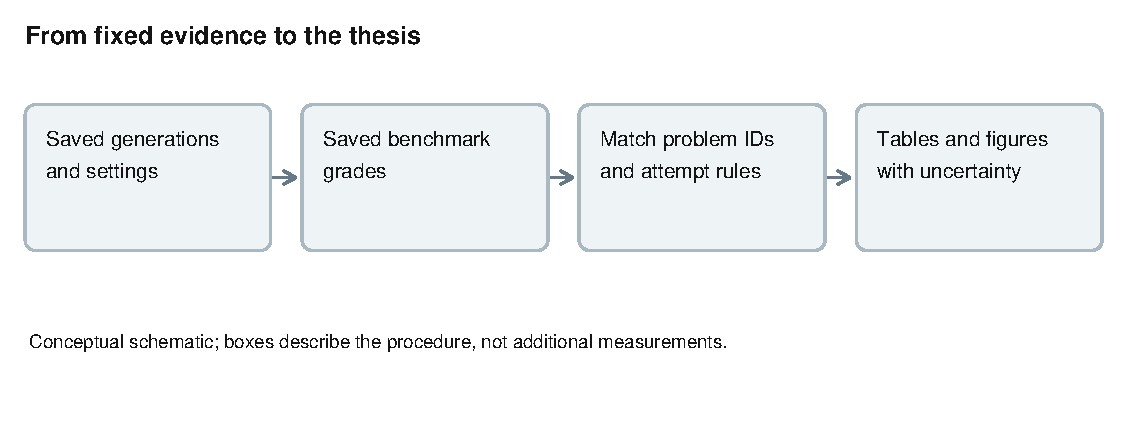
\includegraphics[width=\linewidth]{figures/workflow.pdf}\captionof{figure}{Reporting pipeline. The document build reads historical outputs and grades; it performs no new model generation.}\label{fig:workflow}\end{minipage}\end{center}

The design has two levels. At the experiment level, each configuration specifies a model, an add-on state, and a thinking policy. At the analysis level, the report specifies the covered IDs, attempt rule, outcome calculation, and uncertainty method. A result is interpretable only when both levels are known. For example, a 464-problem one-attempt score and a 234-problem two-attempt average cannot be ranked as if they were the same measurement.\par

\subsection*{3.2 Models and Software}\addcontentsline{toc}{subsection}{3.2 Models and Software}

The study uses Qwen3.5-0.8B, Qwen3.5-2B, and Qwen3.5-4B checkpoints. These are members of the same family, which reduces some variation in interface and model lineage. It does not make the sizes identical systems or isolate model size as the only changing factor. The results describe the specific checkpoints and saved configurations.\par

The saved completed-control environment records Python 3.13.15, PyTorch 2.9.1 with CUDA 12.8, Transformers 5.18.0, PEFT 0.21.1, Flash Linear Attention 0.5.2, and causal-conv1d 1.7.0. Model calculations used bfloat16. These values describe that recorded environment, not a requirement that every historical reference used the same package set. Full environment records remain alongside the raw runs.\par

Notebook 24 records an A100 80GB accelerator and requested a batch size of 128, with the possibility of reducing batches when needed. A batch request is not proof that every generated example was processed in the same batch shape. Since batch layout and numerical kernels can affect sampled outputs, the historical environment difference remains a limitation even where prompts and seeds match.\par

The adapter files record their model association, rank, scaling, and target modules. For the saved 0.8B and 4B LoRA-1 adapters, rank and alpha are both 16 and dropout is zero. These values are read from their configurations rather than assumed from a generic LoRA tutorial. The report preserves the distinction between adapters trained for different base models.\par

\begingroup\singlespacing\small\setlength{\tabcolsep}{4pt}
\begin{longtable}{|p{1.997in}|p{1.997in}|p{1.997in}|}
\caption{Recorded software and experimental resources}\label{tab:software}\\
\hline
\textbf{Item} & \textbf{Recorded value} & \textbf{Scope}\\\hline
\endfirsthead
\hline
\textbf{Item} & \textbf{Recorded value} & \textbf{Scope}\\\hline
\endhead
Models & Qwen3.5 0.8B, 2B, 4B & Three tested sizes\\\hline
Accelerator & A100 80GB & Notebook 24\\\hline
Python / PyTorch & 3.13.15 / 2.9.1+cu128 & Completed-control environment\\\hline
Transformers / PEFT & 5.18.0 / 0.21.1 & Completed-control environment\\\hline
FLA / causal-conv1d & 0.5.2 / 1.7.0 & Completed-control environment\\\hline
Precision & bfloat16 & Recorded calculations\\\hline
Sampling & T=0.6, p=0.95, k=20 & Saved settings\\\hline
Seed & 3407 & Generation and analysis records\\\hline
\end{longtable}
\endgroup

\subsection*{3.3 Test Datasets and Collection}\addcontentsline{toc}{subsection}{3.3 Test Datasets and Collection}

The complete test collection consists of 164 HumanEval+ tasks and 300 LiveCodeBench tasks. Of the contest tasks, 166 are labeled easy and 134 medium. The total is therefore 164 + 166 + 134 = 464. Each problem has a stable ID, allowing matching across methods and detection of duplicate entries. Counts are calculated on unique IDs rather than summed blindly from every file.\par

\begin{center}\begin{minipage}{\linewidth}\centering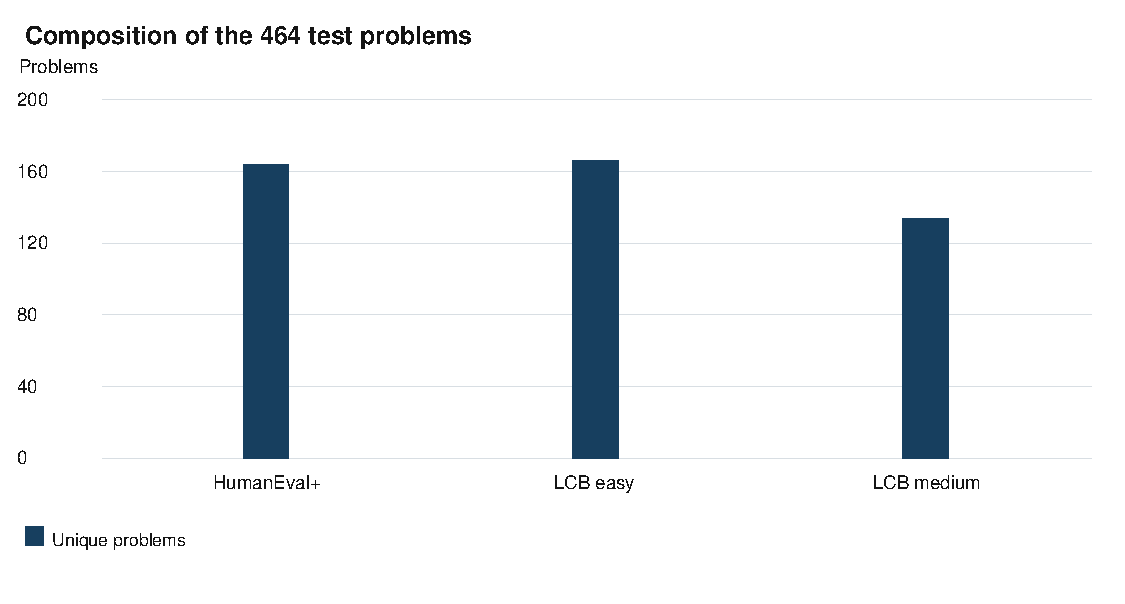
\includegraphics[width=\linewidth]{figures/dataset.pdf}\captionof{figure}{The main test collection has 164 HumanEval+, 166 LiveCodeBench easy, and 134 LiveCodeBench medium tasks.}\label{fig:dataset}\end{minipage}\end{center}

HumanEval+ generally asks the system to complete a Python function. LiveCodeBench tasks include contest-style programs and class methods. These interfaces require different forms of answer extraction and execution. The analysis preserves benchmark groups because interface and difficulty differences can influence observed performance. It does not attribute every group difference to algorithmic reasoning alone.\par

No hard contest tasks are included. This limits the population to which the findings can be applied. The selected easy and medium tasks are still informative about everyday code generation, but they do not establish that a control scales to advanced contests or large software repositories. The 464 problems are the measured collection, not a random draw from all possible programming work.\par

The saved audit reports no duplicated test IDs in the final union. This is a structural check, not a claim that every problem is semantically unrelated. Two distinct tasks may share an algorithm, and similar wording may occur across benchmarks. Such dependencies can reduce the diversity of the evaluation even when ID uniqueness is perfect.\par

\subsection*{3.4 Training Pools and Shortest Correct Selection}\addcontentsline{toc}{subsection}{3.4 Training Pools and Shortest Correct Selection}

LoRA-1 begins from a pool of 100 easy function problems. For each practice problem, the procedure samples candidate answers with thinking enabled, checks correctness, and selects a short successful example where one is available. The retained example count can be smaller than the pool because some problems produce no passing candidate. The saved audit contains 37 retained LoRA-1 examples for 0.8B and 73 for 4B. These are model-specific retained sets, not the full pool size.\par

The historical LoRA-2 procedure uses a larger 280-problem pool: 200 MBPP+ function tasks and 80 older LiveCodeBench tasks, split into 40 easy and 40 medium. Four candidate attempts per problem produce 800 MBPP+ and 320 contest answers. The saved summary reports 357 correct MBPP+ candidates and 44 correct contest candidates. Selection retains 133 function examples and 24 contest examples, making 157 training examples in total.\par

\begin{center}\begin{minipage}{\linewidth}\centering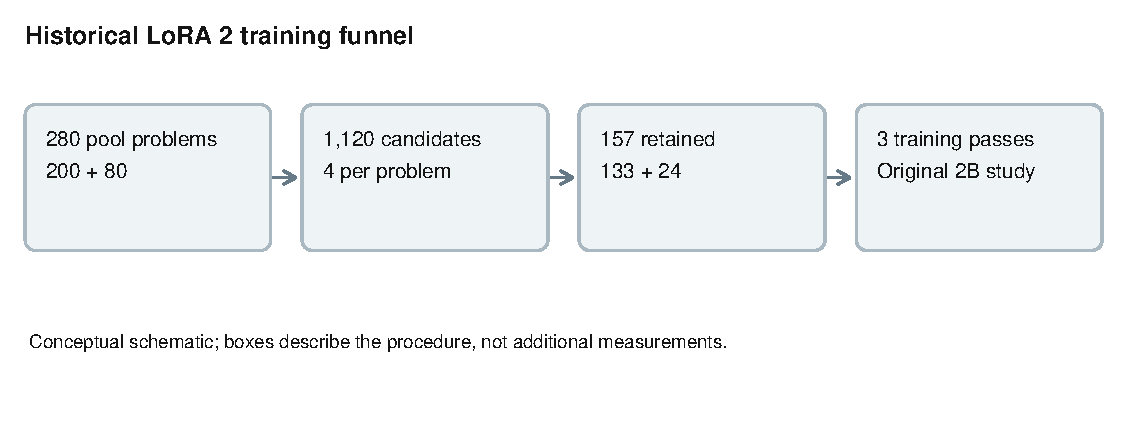
\includegraphics[width=\linewidth]{figures/training.pdf}\captionof{figure}{The historical LoRA-2 funnel retains 157 examples from a 280-problem pool. It is separate from LoRA-1 and the full-set combinations.}\label{fig:training}\end{minipage}\end{center}

The selection rule seeks the shortest correct candidate while applying the saved guard against choosing an answer shorter than half the middle correct length. The purpose is to avoid an extreme short target. This rule is part of the historical method and must not be quietly replaced by a different filtering procedure in the report. Where the saved experiment has only one successful candidate, there is correspondingly little freedom to choose a shorter successful strategy.\par

The retained LoRA-2 function examples have a median thinking length of 515 tokens, while the retained contest examples have a median of 4,709. The selected length divided by average correct length is reported as 0.83 for the function material and 0.99 for the older contest material. The latter leaves little measured compression in that training source. This describes the retained examples; it is not proof that no concise contest solution exists.\par

LoRA-2 trained for three passes over its 157 examples. The saved summary reports about six minutes of training and a loss decrease from about 0.25 to about 0.16. These historical values are approximate and have their original scope. They indicate that training fit changed, while the independent test results determine whether the desired response behavior transferred.\par

Training and test problems are kept separate in the ID audit. The audit compares 280 saved training-pool IDs with the final test IDs and also checks candidate and retained-example files. Exact overlap is zero. Earlier function-name and five-word exclusions remain part of the historical record. This report does not claim a newly completed semantic-overlap audit of all training and test text.\par

\subsection*{3.5 Inference Configurations}\addcontentsline{toc}{subsection}{3.5 Inference Configurations}

Thinking ON permits explicit notes until generation ends or the overall cap is reached. Thinking OFF asks for an answer without explicit thinking notes. A thinking limit stops the notes at the chosen budget and then allows answer generation. A brief prompt asks for concise reasoning through text instructions. These policies are distinct experimental conditions.\par

LoRA-1 alone means the saved add-on with thinking ON and no extra thinking-token limit. LoRA-1 plus OFF uses the same add-on with explicit thinking disabled. LoRA-1 plus limit uses the add-on with the selected budget. The completed budgets are 512 thinking tokens for 0.8B, 1,024 for 2B, and 2,048 for 4B. The numbers apply to thinking, not to the complete output.\par

The total output caps are 4,096 tokens for HumanEval+ and 8,192 for LiveCodeBench. A 512-token thinking limit can therefore be followed by several thousand answer tokens. This distinction helps explain why a model with limited thinking can still have a large total output. For example, a short note section does not prevent a long or repeated answer section.\par

Sampling uses temperature 0.6, top-p 0.95, top-k 20, and seed 3407 in the saved completed-control settings. These choices preserve stochastic generation rather than making every answer a deterministic greedy decode. The same seed is useful provenance, but it does not guarantee identical sampled answers after changing packages, batching, or hardware behavior.\par

Repeat stopping is enabled in the 0.8B and 4B extensions, while 2B retains its original handling. This is an important comparability limit. A cross-size chart is a summary of the actual systems tested, not an experiment that varies parameter count and holds all stopping behavior constant. Within-size paired comparisons remain useful, subject to their historical reference differences.\par

\begingroup\singlespacing\small\setlength{\tabcolsep}{4pt}
\begin{longtable}{|p{1.997in}|p{1.997in}|p{1.997in}|}
\caption{Experimental policies and their interpretation}\label{tab:policies}\\
\hline
\textbf{Policy} & \textbf{Training} & \textbf{Explicit notes}\\\hline
\endfirsthead
\hline
\textbf{Policy} & \textbf{Training} & \textbf{Explicit notes}\\\hline
\endhead
ON & None & Allowed until stopping or output cap\\\hline
OFF & None & Disabled\\\hline
Limit & None & Budgeted before answer\\\hline
Brief prompt & None & Requested concise by wording\\\hline
LoRA alone & LoRA-1 & ON without extra thinking limit\\\hline
LoRA + OFF & Same LoRA-1 & Disabled\\\hline
LoRA + limit & Same LoRA-1 & 512 / 1,024 / 2,048 by size\\\hline
LoRA-2 & Different historical add-on & Original 234-problem study\\\hline
\end{longtable}
\endgroup

\subsection*{3.6 Answer Extraction and Grading}\addcontentsline{toc}{subsection}{3.6 Answer Extraction and Grading}

The saved generation pipeline produces text, from which runnable code is extracted. The grader then evaluates the extracted code in a separate process under time limits. A pass is recorded only when the code succeeds on every test actually used for that attempt. A missing answer, an execution failure, or an incorrect output is not converted into a successful sample by reading a persuasive explanation.\par

HumanEval+ uses the extended tests from its evaluation framework. The saved LiveCodeBench runs use up to 20 tests per problem. This means that the report's LiveCodeBench accuracy should not be described as performance on every hidden test available in the full benchmark. The testing cap is part of the operational definition of success in this study.\par

This document build reads grades rather than running model-generated programs. The approach supports repeatable reporting from the saved evidence. It also means the report does not independently verify every historical grader decision through new execution. The numerical audit checks structural consistency, source hashes where recorded, and recalculated summaries; it does not replace the original execution environment.\par

Code extraction is part of the measured system. A model can fail because it never reaches its final answer, because the extracted answer has the wrong interface, or because the code computes the wrong result. The aggregate pass/fail tables do not separately identify all of these causes. Causal explanations about failure type are therefore limited to analyses that actually inspect the relevant saved content.\par

\subsection*{3.7 Accuracy and Equal Problem Weight}\addcontentsline{toc}{subsection}{3.7 Accuracy and Equal Problem Weight}

Let y(i,j) be 1 when attempt j on problem i passes and 0 otherwise. Let n(i) be the number of available attempts on that problem. Its success fraction is p(i) = sum of y(i,j) divided by n(i). For a method with N covered problems, the combined accuracy is A = sum of p(i) divided by N. This gives each problem equal influence after its available attempts are summarized.\par

\begin{center}\begin{minipage}{\linewidth}\centering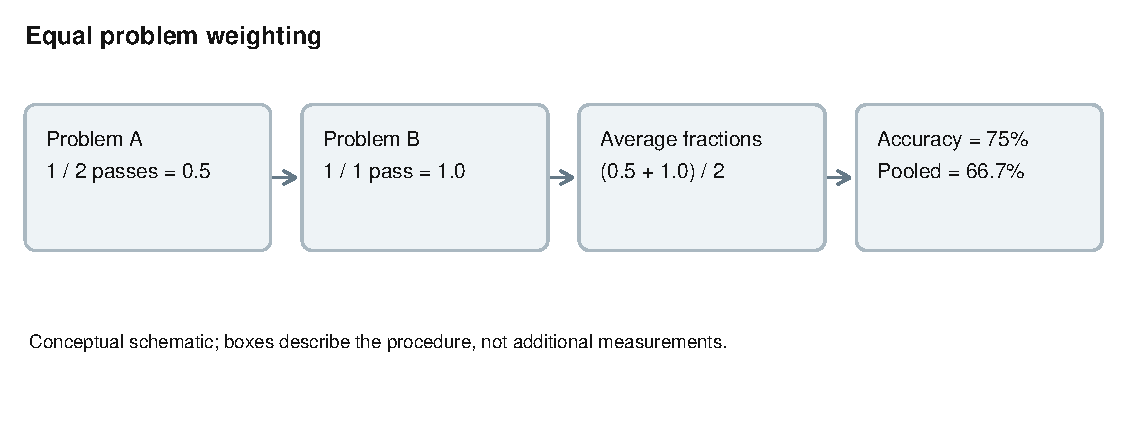
\includegraphics[width=\linewidth]{figures/weighting.pdf}\captionof{figure}{Illustrative arithmetic showing equal problem weighting. These two example problems are not observations from the benchmark.}\label{fig:weighting}\end{minipage}\end{center}

Consider an illustrative two-problem example. Problem A has one pass and one failure, so its fraction is 0.5. Problem B has a single passing attempt, so its fraction is 1.0. Equal problem weighting gives (0.5 + 1.0)/2 = 0.75. Pooling all attempts instead gives 2/3. The example is explanatory arithmetic, not a measured subset of the study.\par

Equal weighting addresses unequal contribution by problem. It does not make the uncertainty of a one-attempt problem identical to that of a repeatedly sampled problem, and it does not remove historical differences in sampling. The report uses it as a transparent summary rule rather than a cure for every feature of the collection. Attempt counts remain visible in result tables.\par

Coverage is the number of unique problems with results for that method. Missing problems are excluded from that method's summary and never counted as failures. For a direct comparison, the relevant set is the intersection of covered IDs. A higher percentage on a smaller, easier subset cannot establish a better score on the full 464-problem collection.\par

\subsection*{3.8 First Attempt Comparisons}\addcontentsline{toc}{subsection}{3.8 First Attempt Comparisons}

Each completed LoRA combination has exactly one attempt per problem. To compare it with a historical control, the completed-control analysis uses that control's saved first attempt on the same IDs. This yields a clearly defined one-answer comparison. It avoids comparing a new single attempt with an older average and calling both values the same kind of single-shot score.\par

The all-attempt summary is retained because it uses the available repeated evidence. Its values may differ from first-attempt accuracy. For instance, 4B limit 2,048 is 71.9\% in the equal-problem all-attempt view and 71.1\% in the first-attempt reference. Both can be correct. The method name is the same, while the estimator and selected attempts differ.\par

The same distinction applies to 2B LoRA-1 alone: its all-attempt score is 34.4\%, while the completed first-attempt comparison uses 34.9\%. These differences are explained at the point of use. They must not be hidden as rounding or reconciled by replacing one estimator with another after looking at which result is more favorable.\par

\subsection*{3.9 Paired Uncertainty Analysis}\addcontentsline{toc}{subsection}{3.9 Paired Uncertainty Analysis}

The saved analyses use 2,000 bootstrap replicates with seed 3407. A bootstrap replicate samples whole problems with replacement from the relevant shared set and recomputes the statistic. For a difference, both methods stay attached to the same sampled problem. The 2.5th and 97.5th percentiles form the reported 95\% interval.\par

\begin{center}\begin{minipage}{\linewidth}\centering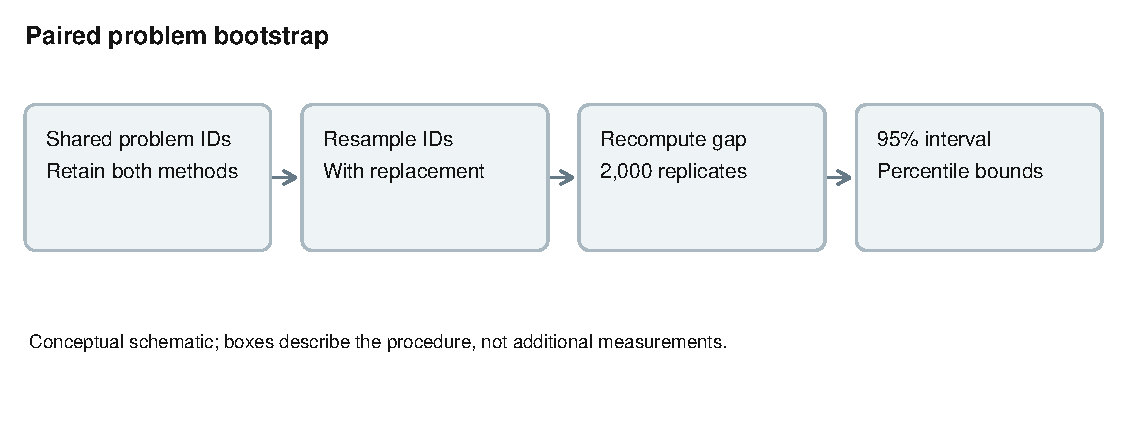
\includegraphics[width=\linewidth]{figures/bootstrap.pdf}\captionof{figure}{The saved uncertainty procedure resamples problems while retaining each paired comparison. Intervals are unadjusted.}\label{fig:bootstrap}\end{minipage}\end{center}

Pairing is useful because a difficult problem can affect both methods. Comparing the methods on the same resampled IDs keeps that shared difficulty in the difference calculation. Sampling individual attempts as if they were unrelated problems would instead overstate the amount of independent information when attempts are repeated within a task.\par

These intervals describe variation over the observed problem collection under the saved procedure. They do not include all uncertainty from training seeds, future prompts, package changes, or a different distribution of programming work. They are also unadjusted for multiple comparisons and for choosing interesting methods after results were seen. A positive interval is evidence within this analysis, not a universal guarantee.\par

When an interval includes zero, the report calls the measured gain uncertain or inconclusive. That does not prove the methods are equivalent. Equivalence would require a prespecified acceptable margin and an appropriate design. When an interval excludes zero, the direction is reported along with the same retrospective and multiplicity limitations.\par

\subsection*{3.10 Tokens, Cap Hits, and Resource Reporting}\addcontentsline{toc}{subsection}{3.10 Tokens, Cap Hits, and Resource Reporting}

Thinking tokens measure the explicit notes portion. Total new tokens measure the full generated response counted by the saved pipeline. OFF records zero thinking tokens but can still generate a long answer. A thinking limit is therefore evaluated against both components rather than assumed to control the total response perfectly.\par

Token summaries use the saved problem-based averaging convention. The report does not infer GPU speed from tokens alone. A larger model can take different time per token, and a different batch layout can change throughput. Training and candidate generation add an up-front resource requirement that is not captured by inference output length.\par

A cap hit is the saved indicator that an output reached the overall maximum. It does not by itself diagnose repetition. The original 234-problem analysis separately investigated loops in capped 2B outputs. Those values are reported as historical diagnostics. The full-coverage cap-rate figures show only the cap event measured for their corresponding configurations.\par

Notebook 24's ledger estimates about 57.0 Colab units for its five runs. This is a local record of that extension, not a complete project cost statement. It excludes the earlier 2B combination and other work. The number must not be converted into hours without a stated rate, or described as an externally verified bill.\par

\subsection*{3.11 Validation and Reproducibility}\addcontentsline{toc}{subsection}{3.11 Validation and Reproducibility}

Validation begins with IDs. Each completed configuration must contain the expected 464 unique IDs, exactly one raw answer per ID, and a corresponding grade. Unexpected IDs or duplicate attempts would invalidate a simple 464-denominator calculation. The completed archive checks report that these structural conditions are satisfied.\par

The next layer checks model settings, thinking policy, adapter hashes, raw/graded token agreement, and the historical reference manifests. These checks reduce the risk of labeling one run as another. Hashes establish identity of files, not scientific correctness of their contents. They must be interpreted as provenance controls rather than proof that a model answer is right.\par

The numerical layer recalculates percentages and paired differences from the saved records. This thesis builds its tables and plots from the checked JSON summaries and records their source hashes in the delivery package. Assertions verify the main sample counts and completed-combination pass totals. The appendices identify the source files and local reproduction commands.\par

The reporting layer checks whether text, figures, and tables use the same estimator and denominator. It also checks whether a result from a partial method is labeled with its actual coverage. This is a scientific validation step because inconsistent captions can create a false claim even when every number was copied correctly.\par

\subsection*{3.12 Chapter Summary}\addcontentsline{toc}{subsection}{3.12 Chapter Summary}

The methodology uses fixed saved evidence, unique problem IDs, clearly defined estimators, and paired uncertainty intervals. Its strongest comparisons are those with matched problems and explicit attempt rules. Its main limitations are retrospective selection, historical environment differences, restricted benchmark coverage, and incomplete measurement of resource costs. Chapter 4 presents the numerical outcomes under these definitions.\par

\clearpage

\section*{Chapter 4: Results}\addcontentsline{toc}{section}{Chapter 4: Results}

\subsection*{4.1 Reading the Results}\addcontentsline{toc}{subsection}{4.1 Reading the Results}

This chapter reports measurements before interpreting their possible causes. The full-coverage tables use equal problem weighting across available attempts. The completed-control tables identify first-attempt comparisons explicitly. Every full-coverage row covers 464 unique problems. Partial sweeps and historical diagnostics appear separately with their original scope.\par

The checked result summaries supply the numeric values used in this chapter. Percentages are rounded only for display. A rounded percentage multiplied by a denominator may not recover an integer pass total in the all-attempt view because individual problem scores can be fractions. Integer passed counts are therefore given only where the configuration has one answer per problem.\par

The 95\% intervals use the saved problem bootstrap procedure. They do not correct for multiple comparisons or for selection after viewing results. Where an interval on a difference includes zero, the result is described as uncertain. All token counts refer to generated output, not to elapsed time or billed cost.\par

\begin{center}\begin{minipage}{\linewidth}\centering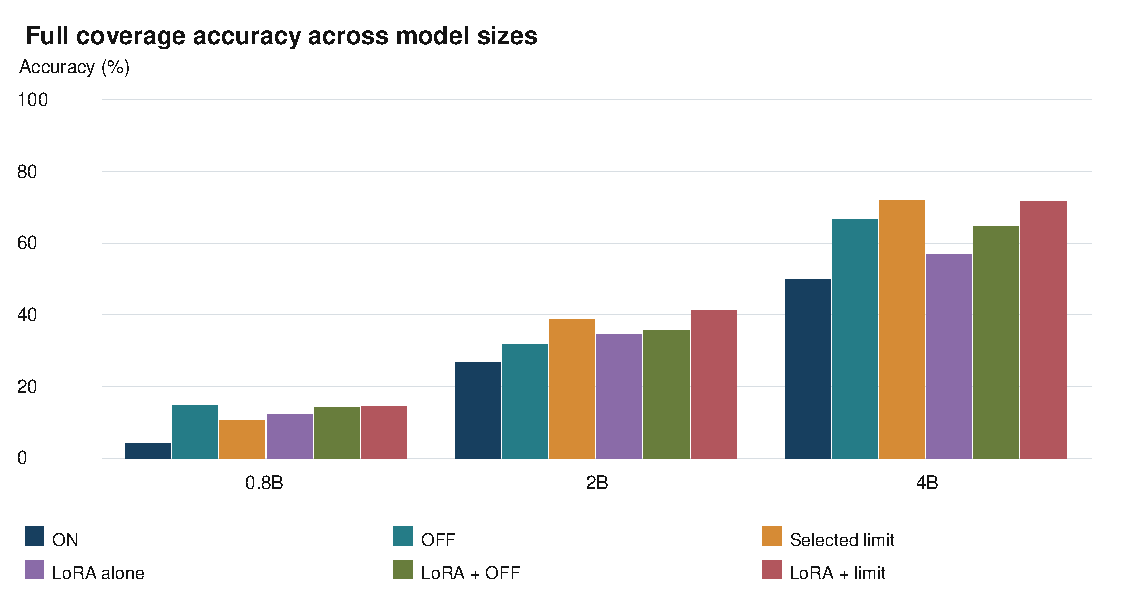
\includegraphics[width=\linewidth]{figures/accuracy.pdf}\captionof{figure}{Accuracy uses equal problem weights over all available attempts on 464 problems per method. Selected limits are 512, 1,024, and 2,048 by size.}\label{fig:accuracy}\end{minipage}\end{center}

\subsection*{4.2 Full Coverage Results for 0.8B}\addcontentsline{toc}{subsection}{4.2 Full Coverage Results for 0.8B}

Table \ref{tab:fullX0X8b} reports the six complete configurations for Qwen3.5-0.8B. All use the same 464 problem IDs, while the number of saved attempts varies by historical method. The table states the attempt total, accuracy, percentile interval, and mean total output tokens. It is the all-attempt equal-problem summary, rather than a first-attempt ranking.\par

\begingroup\singlespacing\small\setlength{\tabcolsep}{4pt}
\begin{longtable}{|p{1.130in}|p{1.130in}|p{1.130in}|p{1.130in}|p{1.130in}|}
\caption{Qwen3.5-0.8B full coverage with equal problem weighting}\label{tab:fullX0X8b}\\
\hline
\textbf{Method} & \textbf{Attempts} & \textbf{Accuracy} & \textbf{95\% interval} & \textbf{Total tokens}\\\hline
\endfirsthead
\hline
\textbf{Method} & \textbf{Attempts} & \textbf{Accuracy} & \textbf{95\% interval} & \textbf{Total tokens}\\\hline
\endhead
ON & 464 & 4.1\% & [2.4\%, 6.0\%] & 6,206\\\hline
OFF & 464 & 14.7\% & [11.6\%, 17.9\%] & 1,781\\\hline
Limit 512 & 464 & 10.6\% & [7.8\%, 13.6\%] & 5,920\\\hline
LoRA alone & 464 & 12.3\% & [9.3\%, 15.3\%] & 5,256\\\hline
LoRA + OFF & 464 & 14.0\% & [11.0\%, 17.0\%] & 1,278\\\hline
LoRA + Limit  512 & 464 & 14.4\% & [11.2\%, 17.5\%] & 4,979\\\hline
\end{longtable}
\endgroup

Unrestricted ON records 4.1\% accuracy and 6,206 mean total tokens. OFF records 14.7\% and 1,781 tokens. The selected free limit of 512 thinking tokens records 10.6\% and 5,920 total tokens. These values describe complete response lengths, so the total can exceed the stated thinking budget.\par

LoRA alone records 12.3\% with 464 saved attempts on the 464 problems. LoRA plus OFF records 14.0\%, while LoRA plus the selected limit records 14.4\%. Both combinations have 464 attempts, one per problem. Their results can be read as integer counts in the completed-combination table later in this chapter.\par

The table does not establish a universal winner. It lists the measured policies on the complete collection. A decision about whether training helps needs the corresponding paired comparison and its attempt rule, rather than a subtraction between arbitrary rows. The benchmark breakdown in Figure \ref{fig:groups0X8b} shows how the combined result is distributed across task groups.\par

\begin{center}\begin{minipage}{\linewidth}\centering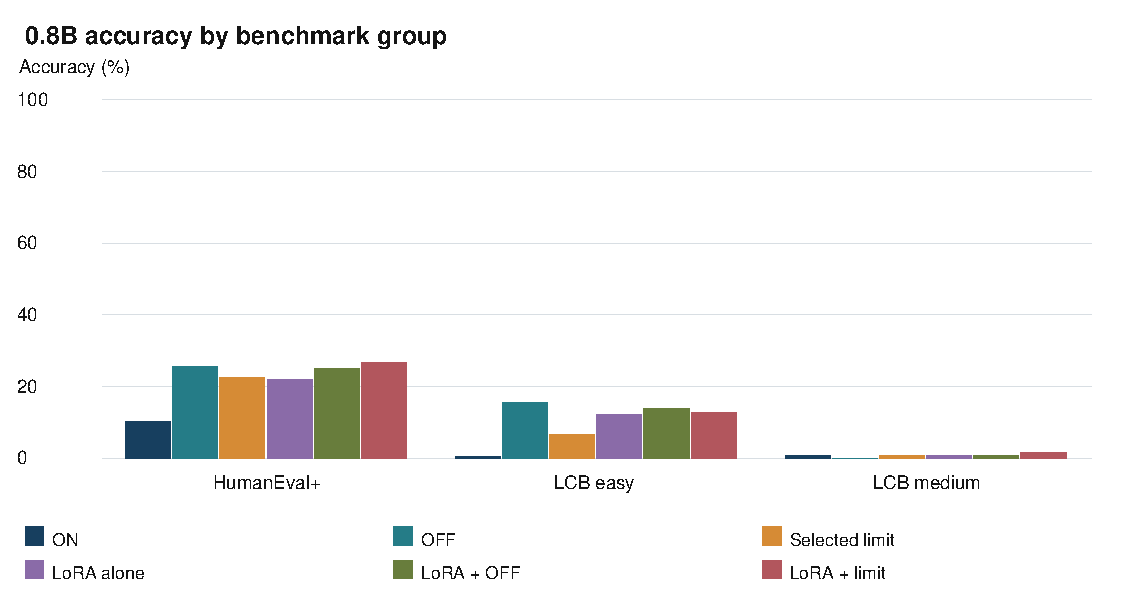
\includegraphics[width=\linewidth]{figures/groups0.8b.pdf}\captionof{figure}{0.8B benchmark breakdown, using all-attempt equal-problem accuracy. Group sizes are 164, 166, and 134. No hard contest tasks are included.}\label{fig:groups0X8b}\end{minipage}\end{center}

\begingroup\singlespacing\small\setlength{\tabcolsep}{4pt}
\begin{longtable}{|p{1.455in}|p{1.455in}|p{1.455in}|p{1.455in}|}
\caption{0.8B accuracy by benchmark group using all available attempts}\label{tab:groupsX0X8b}\\
\hline
\textbf{Method} & \textbf{HumanEval+ 164} & \textbf{LCB easy 166} & \textbf{LCB medium 134}\\\hline
\endfirsthead
\hline
\textbf{Method} & \textbf{HumanEval+ 164} & \textbf{LCB easy 166} & \textbf{LCB medium 134}\\\hline
\endhead
ON & 10.4\% & 0.6\% & 0.7\%\\\hline
OFF & 25.6\% & 15.7\% & 0.0\%\\\hline
Limit 512 & 22.6\% & 6.6\% & 0.7\%\\\hline
LoRA alone & 22.0\% & 12.0\% & 0.7\%\\\hline
LoRA + OFF & 25.0\% & 13.9\% & 0.7\%\\\hline
LoRA + Limit  512 & 26.8\% & 12.7\% & 1.5\%\\\hline
\end{longtable}
\endgroup

Within HumanEval+, the highest observed value among these six complete methods is 26.8\% for LoRA + Limit  512. The lowest is 10.4\% for ON. This is a descriptive comparison within 164 problems, not a separate set of experiments. Ties and uncertainty can make an ordered ranking less informative than the displayed values themselves.\par

Within LiveCodeBench easy, the highest observed value among these six complete methods is 15.7\% for OFF. The lowest is 0.6\% for ON. This is a descriptive comparison within 166 problems, not a separate set of experiments. Ties and uncertainty can make an ordered ranking less informative than the displayed values themselves.\par

Within LiveCodeBench medium, the highest observed value among these six complete methods is 1.5\% for LoRA + Limit  512. The lowest is 0.0\% for OFF. This is a descriptive comparison within 134 problems, not a separate set of experiments. Ties and uncertainty can make an ordered ranking less informative than the displayed values themselves.\par

The small medium-task percentages deserve attention alongside the combined 0.8B score. A policy can increase success on functions while leaving contest performance very limited. The benchmark interfaces and task demands differ, so these group results locate the weakness without isolating its cause. The overall uncertainty interval is not a subgroup interval.\par

\subsection*{4.3 Full Coverage Results for 2B}\addcontentsline{toc}{subsection}{4.3 Full Coverage Results for 2B}

Table \ref{tab:fullX2b} reports the six complete configurations for Qwen3.5-2B. All use the same 464 problem IDs, while the number of saved attempts varies by historical method. The table states the attempt total, accuracy, percentile interval, and mean total output tokens. It is the all-attempt equal-problem summary, rather than a first-attempt ranking.\par

\begingroup\singlespacing\small\setlength{\tabcolsep}{4pt}
\begin{longtable}{|p{1.130in}|p{1.130in}|p{1.130in}|p{1.130in}|p{1.130in}|}
\caption{Qwen3.5-2B full coverage with equal problem weighting}\label{tab:fullX2b}\\
\hline
\textbf{Method} & \textbf{Attempts} & \textbf{Accuracy} & \textbf{95\% interval} & \textbf{Total tokens}\\\hline
\endfirsthead
\hline
\textbf{Method} & \textbf{Attempts} & \textbf{Accuracy} & \textbf{95\% interval} & \textbf{Total tokens}\\\hline
\endhead
ON & 738 & 26.8\% & [23.2\%, 30.6\%] & 5,331\\\hline
OFF & 738 & 31.8\% & [27.7\%, 36.0\%] & 1,337\\\hline
Limit 1024 & 738 & 38.6\% & [34.4\%, 42.8\%] & 4,337\\\hline
LoRA alone & 698 & 34.4\% & [30.3\%, 38.4\%] & 4,735\\\hline
LoRA + OFF & 464 & 35.6\% & [31.2\%, 39.7\%] & 1,445\\\hline
LoRA + Limit  1024 & 464 & 41.2\% & [36.6\%, 45.7\%] & 4,072\\\hline
\end{longtable}
\endgroup

Unrestricted ON records 26.8\% accuracy and 5,331 mean total tokens. OFF records 31.8\% and 1,337 tokens. The selected free limit of 1,024 thinking tokens records 38.6\% and 4,337 total tokens. These values describe complete response lengths, so the total can exceed the stated thinking budget.\par

LoRA alone records 34.4\% with 698 saved attempts on the 464 problems. LoRA plus OFF records 35.6\%, while LoRA plus the selected limit records 41.2\%. Both combinations have 464 attempts, one per problem. Their results can be read as integer counts in the completed-combination table later in this chapter.\par

The table does not establish a universal winner. It lists the measured policies on the complete collection. A decision about whether training helps needs the corresponding paired comparison and its attempt rule, rather than a subtraction between arbitrary rows. The benchmark breakdown in Figure \ref{fig:groups2b} shows how the combined result is distributed across task groups.\par

\begin{center}\begin{minipage}{\linewidth}\centering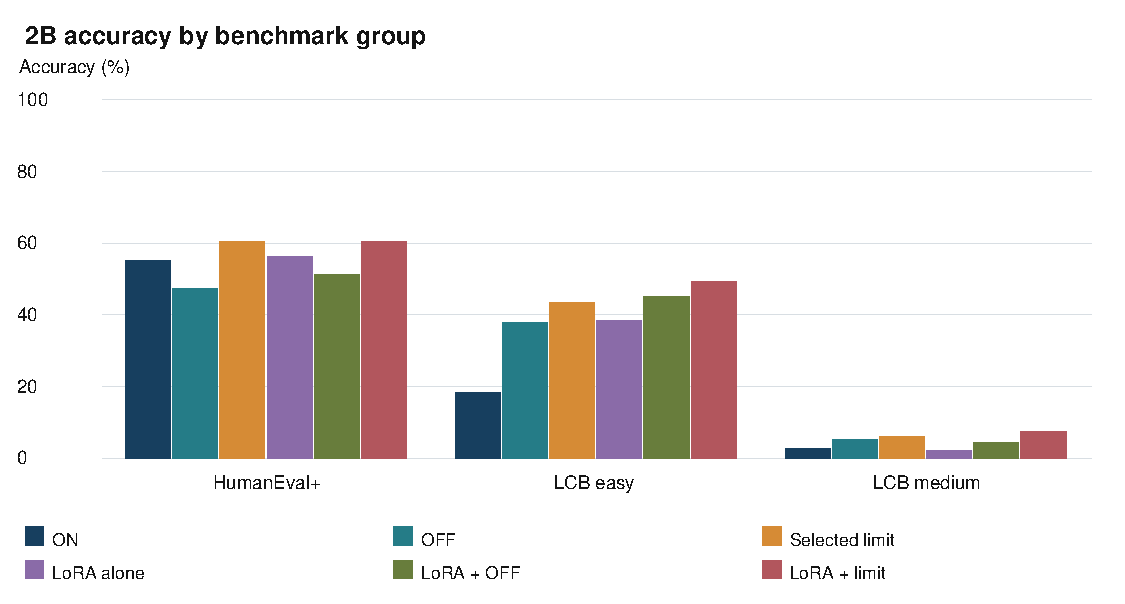
\includegraphics[width=\linewidth]{figures/groups2b.pdf}\captionof{figure}{2B benchmark breakdown, using all-attempt equal-problem accuracy. Group sizes are 164, 166, and 134. No hard contest tasks are included.}\label{fig:groups2b}\end{minipage}\end{center}

\begingroup\singlespacing\small\setlength{\tabcolsep}{4pt}
\begin{longtable}{|p{1.455in}|p{1.455in}|p{1.455in}|p{1.455in}|}
\caption{2B accuracy by benchmark group using all available attempts}\label{tab:groupsX2b}\\
\hline
\textbf{Method} & \textbf{HumanEval+ 164} & \textbf{LCB easy 166} & \textbf{LCB medium 134}\\\hline
\endfirsthead
\hline
\textbf{Method} & \textbf{HumanEval+ 164} & \textbf{LCB easy 166} & \textbf{LCB medium 134}\\\hline
\endhead
ON & 55.2\% & 18.4\% & 2.6\%\\\hline
OFF & 47.3\% & 38.0\% & 5.2\%\\\hline
Limit 1024 & 60.4\% & 43.4\% & 6.0\%\\\hline
LoRA alone & 56.4\% & 38.6\% & 2.2\%\\\hline
LoRA + OFF & 51.2\% & 45.2\% & 4.5\%\\\hline
LoRA + Limit  1024 & 60.4\% & 49.4\% & 7.5\%\\\hline
\end{longtable}
\endgroup

Within HumanEval+, the highest observed value among these six complete methods is 60.4\% for Limit 1024. The lowest is 47.3\% for OFF. This is a descriptive comparison within 164 problems, not a separate set of experiments. Ties and uncertainty can make an ordered ranking less informative than the displayed values themselves.\par

Within LiveCodeBench easy, the highest observed value among these six complete methods is 49.4\% for LoRA + Limit  1024. The lowest is 18.4\% for ON. This is a descriptive comparison within 166 problems, not a separate set of experiments. Ties and uncertainty can make an ordered ranking less informative than the displayed values themselves.\par

Within LiveCodeBench medium, the highest observed value among these six complete methods is 7.5\% for LoRA + Limit  1024. The lowest is 2.2\% for LoRA alone. This is a descriptive comparison within 134 problems, not a separate set of experiments. Ties and uncertainty can make an ordered ranking less informative than the displayed values themselves.\par

The 2B results show a substantial separation between function tasks and medium contest tasks. That separation remains visible after adding the trained controls. A user whose workload consists mainly of contest programs should inspect those columns before applying a conclusion from the combined score. No unreported subgroup significance test is inferred here.\par

\subsection*{4.4 Full Coverage Results for 4B}\addcontentsline{toc}{subsection}{4.4 Full Coverage Results for 4B}

Table \ref{tab:fullX4b} reports the six complete configurations for Qwen3.5-4B. All use the same 464 problem IDs, while the number of saved attempts varies by historical method. The table states the attempt total, accuracy, percentile interval, and mean total output tokens. It is the all-attempt equal-problem summary, rather than a first-attempt ranking.\par

\begingroup\singlespacing\small\setlength{\tabcolsep}{4pt}
\begin{longtable}{|p{1.130in}|p{1.130in}|p{1.130in}|p{1.130in}|p{1.130in}|}
\caption{Qwen3.5-4B full coverage with equal problem weighting}\label{tab:fullX4b}\\
\hline
\textbf{Method} & \textbf{Attempts} & \textbf{Accuracy} & \textbf{95\% interval} & \textbf{Total tokens}\\\hline
\endfirsthead
\hline
\textbf{Method} & \textbf{Attempts} & \textbf{Accuracy} & \textbf{95\% interval} & \textbf{Total tokens}\\\hline
\endhead
ON & 738 & 50.0\% & [45.9\%, 54.3\%] & 5,188\\\hline
OFF & 738 & 66.5\% & [62.3\%, 70.5\%] & 943\\\hline
Limit 2048 & 738 & 71.9\% & [67.9\%, 75.6\%] & 3,921\\\hline
LoRA alone & 698 & 56.8\% & [52.5\%, 61.0\%] & 4,797\\\hline
LoRA + OFF & 464 & 64.7\% & [59.9\%, 69.0\%] & 882\\\hline
LoRA + Limit  2048 & 464 & 71.6\% & [67.5\%, 75.6\%] & 3,511\\\hline
\end{longtable}
\endgroup

Unrestricted ON records 50.0\% accuracy and 5,188 mean total tokens. OFF records 66.5\% and 943 tokens. The selected free limit of 2,048 thinking tokens records 71.9\% and 3,921 total tokens. These values describe complete response lengths, so the total can exceed the stated thinking budget.\par

LoRA alone records 56.8\% with 698 saved attempts on the 464 problems. LoRA plus OFF records 64.7\%, while LoRA plus the selected limit records 71.6\%. Both combinations have 464 attempts, one per problem. Their results can be read as integer counts in the completed-combination table later in this chapter.\par

The table does not establish a universal winner. It lists the measured policies on the complete collection. A decision about whether training helps needs the corresponding paired comparison and its attempt rule, rather than a subtraction between arbitrary rows. The benchmark breakdown in Figure \ref{fig:groups4b} shows how the combined result is distributed across task groups.\par

\begin{center}\begin{minipage}{\linewidth}\centering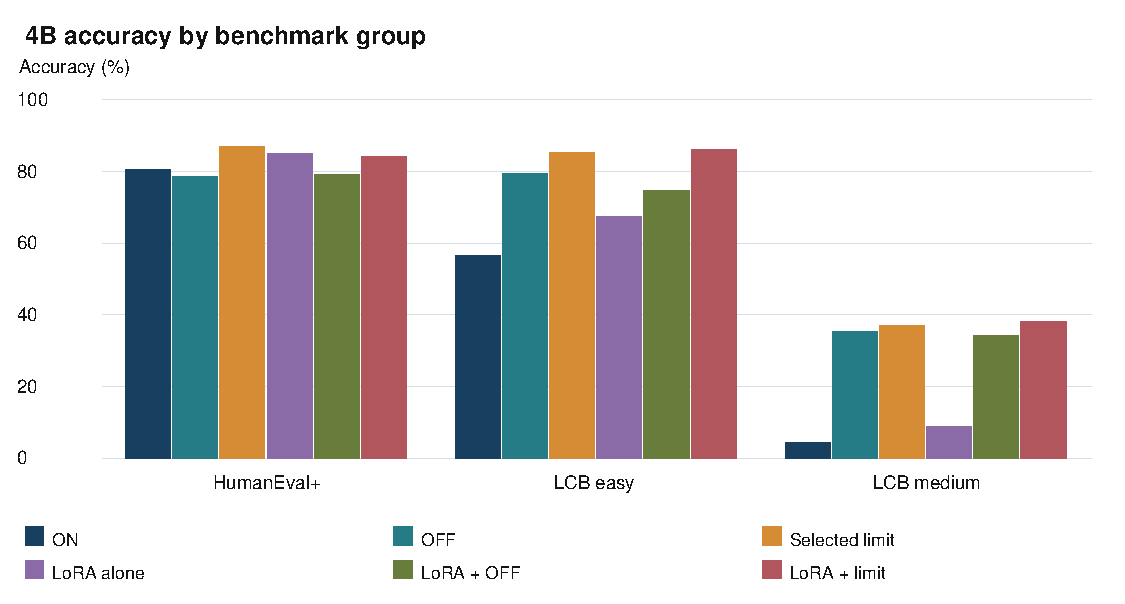
\includegraphics[width=\linewidth]{figures/groups4b.pdf}\captionof{figure}{4B benchmark breakdown, using all-attempt equal-problem accuracy. Group sizes are 164, 166, and 134. No hard contest tasks are included.}\label{fig:groups4b}\end{minipage}\end{center}

\begingroup\singlespacing\small\setlength{\tabcolsep}{4pt}
\begin{longtable}{|p{1.455in}|p{1.455in}|p{1.455in}|p{1.455in}|}
\caption{4B accuracy by benchmark group using all available attempts}\label{tab:groupsX4b}\\
\hline
\textbf{Method} & \textbf{HumanEval+ 164} & \textbf{LCB easy 166} & \textbf{LCB medium 134}\\\hline
\endfirsthead
\hline
\textbf{Method} & \textbf{HumanEval+ 164} & \textbf{LCB easy 166} & \textbf{LCB medium 134}\\\hline
\endhead
ON & 80.5\% & 56.6\% & 4.5\%\\\hline
OFF & 78.7\% & 79.5\% & 35.4\%\\\hline
Limit 2048 & 86.9\% & 85.2\% & 36.9\%\\\hline
LoRA alone & 85.1\% & 67.5\% & 9.0\%\\\hline
LoRA + OFF & 79.3\% & 74.7\% & 34.3\%\\\hline
LoRA + Limit  2048 & 84.1\% & 86.1\% & 38.1\%\\\hline
\end{longtable}
\endgroup

Within HumanEval+, the highest observed value among these six complete methods is 86.9\% for Limit 2048. The lowest is 78.7\% for OFF. This is a descriptive comparison within 164 problems, not a separate set of experiments. Ties and uncertainty can make an ordered ranking less informative than the displayed values themselves.\par

Within LiveCodeBench easy, the highest observed value among these six complete methods is 86.1\% for LoRA + Limit  2048. The lowest is 56.6\% for ON. This is a descriptive comparison within 166 problems, not a separate set of experiments. Ties and uncertainty can make an ordered ranking less informative than the displayed values themselves.\par

Within LiveCodeBench medium, the highest observed value among these six complete methods is 38.1\% for LoRA + Limit  2048. The lowest is 4.5\% for ON. This is a descriptive comparison within 134 problems, not a separate set of experiments. Ties and uncertainty can make an ordered ranking less informative than the displayed values themselves.\par

The 4B model succeeds more often across the displayed groups, but the medium contest tasks remain harder under the tested policies. The group comparison also shows that an advantage on one benchmark need not have the same size on another. These descriptive values use the existing grades and do not add new tests or establish a causal explanation.\par

\subsection*{4.5 Completed LoRA Combinations with One Attempt}\addcontentsline{toc}{subsection}{4.5 Completed LoRA Combinations with One Attempt}

All six planned combinations are finished. Each has one raw answer and one grade for every problem. Five configurations come from Notebook 24 and the 2B limit combination comes from the earlier Notebook 21. This section reports the common one-attempt denominator directly. It does not average the completed-combination scores with older attempts.\par

\begingroup\singlespacing\small\setlength{\tabcolsep}{4pt}
\begin{longtable}{|p{0.913in}|p{0.913in}|p{0.913in}|p{0.913in}|p{0.913in}|p{0.913in}|}
\caption{All six completed combinations with one answer per problem}\label{tab:completed}\\
\hline
\textbf{Size} & \textbf{Combination} & \textbf{Passed} & \textbf{Accuracy} & \textbf{95\% interval} & \textbf{Tokens}\\\hline
\endfirsthead
\hline
\textbf{Size} & \textbf{Combination} & \textbf{Passed} & \textbf{Accuracy} & \textbf{95\% interval} & \textbf{Tokens}\\\hline
\endhead
0.8B & LoRA + OFF & 65/464 & 14.0\% & [11.0\%, 17.0\%] & 1,278\\\hline
0.8B & LoRA + Limit  512 & 67/464 & 14.4\% & [11.2\%, 17.5\%] & 4,979\\\hline
2B & LoRA + OFF & 165/464 & 35.6\% & [31.2\%, 39.7\%] & 1,445\\\hline
2B & LoRA + Limit  1024 & 191/464 & 41.2\% & [36.6\%, 45.7\%] & 4,072\\\hline
4B & LoRA + OFF & 300/464 & 64.7\% & [59.9\%, 69.0\%] & 882\\\hline
4B & LoRA + Limit  2048 & 332/464 & 71.6\% & [67.5\%, 75.6\%] & 3,511\\\hline
\end{longtable}
\endgroup

The totals are 65 and 67 passes for 0.8B, 165 and 191 for 2B, and 300 and 332 for 4B, ordered as OFF then limit. The denominator is the same in every case. These counts establish completion and observed outcomes; they do not by themselves measure an improvement over the untrained policy.\par

The 2B limit combination has the largest observed complete-set accuracy among the tested 2B configurations. The 4B limit combination passes 332 problems and the 0.8B limit combination passes 67. The following paired comparisons determine whether these observations establish a gain beyond their corresponding free controls.\par

\subsection*{4.6 Matched First Attempt Comparisons}\addcontentsline{toc}{subsection}{4.6 Matched First Attempt Comparisons}

This section uses historical first attempts for the references. The control table and forest plot therefore use a different attempt selection from the earlier all-attempt tables. The 4B free limit is 330/464, or 71.1\%, in this view. Its 71.9\% all-attempt score is not substituted into this first-attempt difference.\par

\begingroup\singlespacing\small\setlength{\tabcolsep}{4pt}
\begin{longtable}{|p{1.130in}|p{1.130in}|p{1.130in}|p{1.130in}|p{1.130in}|}
\caption{Training addition versus the matching free policy on first attempts}\label{tab:first}\\
\hline
\textbf{Size / policy} & \textbf{Trained} & \textbf{Free} & \textbf{Gap pp} & \textbf{95\% gap pp}\\\hline
\endfirsthead
\hline
\textbf{Size / policy} & \textbf{Trained} & \textbf{Free} & \textbf{Gap pp} & \textbf{95\% gap pp}\\\hline
\endhead
0.8B OFF & 14.0\% & 14.7\% & -0.6 & [-3.2, 2.2]\\\hline
0.8B limit & 14.4\% & 10.6\% & +3.9 & [0.6, 7.1]\\\hline
2B OFF & 35.6\% & 32.5\% & +3.0 & [-0.6, 6.9]\\\hline
2B limit & 41.2\% & 38.6\% & +2.6 & [-1.5, 6.7]\\\hline
4B OFF & 64.7\% & 66.4\% & -1.7 & [-5.6, 1.9]\\\hline
4B limit & 71.6\% & 71.1\% & +0.4 & [-3.0, 3.7]\\\hline
\end{longtable}
\endgroup

\begin{center}\begin{minipage}{\linewidth}\centering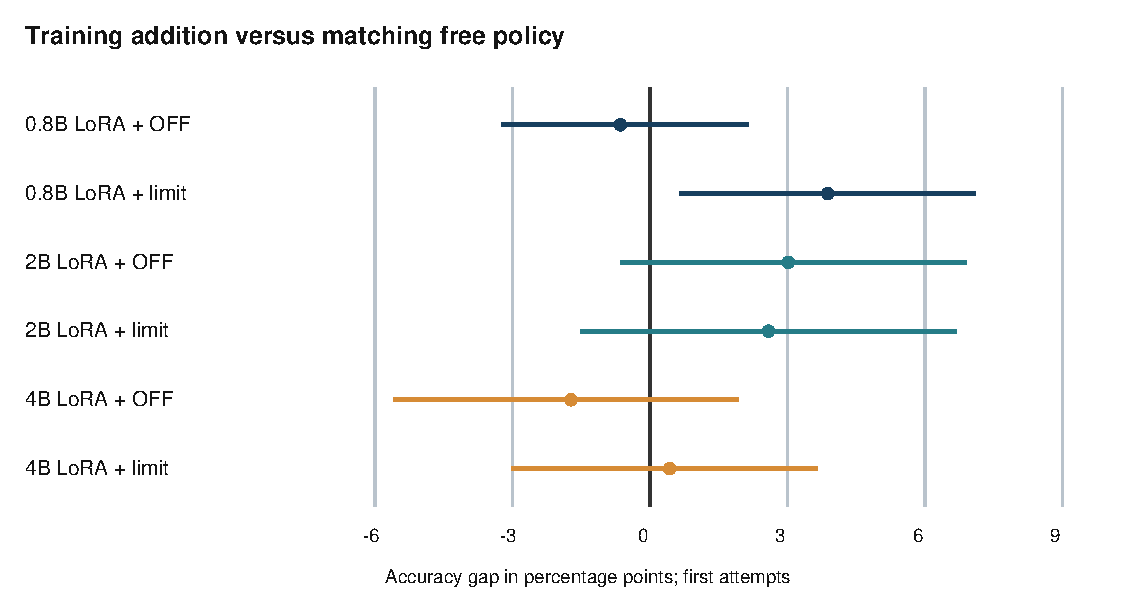
\includegraphics[width=\linewidth]{figures/forest.pdf}\captionof{figure}{Paired first-attempt accuracy differences for each trained policy against the same policy without LoRA. Bars are unadjusted 95\% intervals; crossing zero indicates an inconclusive gain.}\label{fig:forest}\end{minipage}\end{center}

For 0.8B LoRA + OFF, the difference from OFF is -0.6 percentage points, with a paired 95\% interval of [-3.2, 2.2] points. The comparison uses 464 shared problems and the first-attempt reference. The interval includes zero, so a reliable accuracy gain is not established.\par

For 0.8B LoRA + Limit  512, the difference from Limit 512 is +3.9 percentage points, with a paired 95\% interval of [0.6, 7.1] points. The comparison uses 464 shared problems and the first-attempt reference. The interval excludes zero in the positive direction under this unadjusted analysis.\par

For 2B LoRA + OFF, the difference from OFF is +3.0 percentage points, with a paired 95\% interval of [-0.6, 6.9] points. The comparison uses 464 shared problems and the first-attempt reference. The interval includes zero, so a reliable accuracy gain is not established.\par

For 2B LoRA + Limit  1024, the difference from Limit 1024 is +2.6 percentage points, with a paired 95\% interval of [-1.5, 6.7] points. The comparison uses 464 shared problems and the first-attempt reference. The interval includes zero, so a reliable accuracy gain is not established.\par

For 4B LoRA + OFF, the difference from OFF is -1.7 percentage points, with a paired 95\% interval of [-5.6, 1.9] points. The comparison uses 464 shared problems and the first-attempt reference. The interval includes zero, so a reliable accuracy gain is not established.\par

For 4B LoRA + Limit  2048, the difference from Limit 2048 is +0.4 percentage points, with a paired 95\% interval of [-3.0, 3.7] points. The comparison uses 464 shared problems and the first-attempt reference. The interval includes zero, so a reliable accuracy gain is not established.\par

The 2B trained limit exceeds the trained OFF policy by 5.6 points, with an interval of +1.1 to +9.9. This compares two trained configurations. It is evidence about the thinking policy used with the add-on, not proof of the benefit of training over an untrained model.\par

For 4B, the trained limit has two more passes than the free-limit first attempt. The corresponding gap is about +0.4 points, with an interval of -3.0 to +3.7. Both a modest loss and a modest gain remain compatible with this saved comparison. The interval does not establish practical equivalence.\par

\subsection*{4.7 Output Length and Accuracy Tradeoffs}\addcontentsline{toc}{subsection}{4.7 Output Length and Accuracy Tradeoffs}

\begin{center}\begin{minipage}{\linewidth}\centering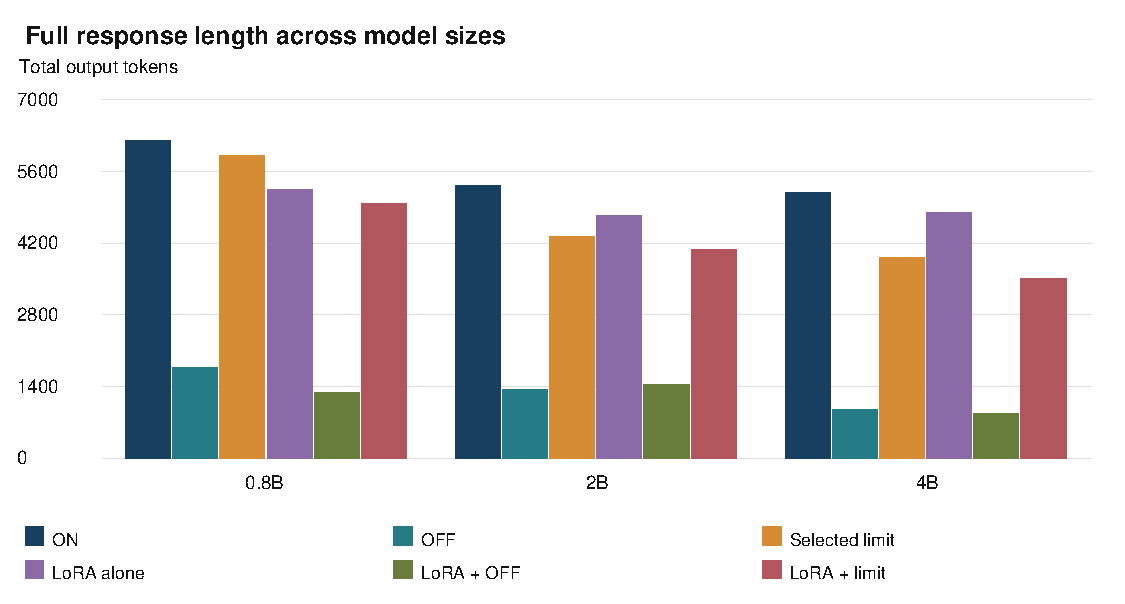
\includegraphics[width=\linewidth]{figures/tokens.pdf}\captionof{figure}{Mean total new tokens with equal problem weighting over available attempts. Thinking budgets do not cap the complete answer.}\label{fig:tokens}\end{minipage}\end{center}

\begin{center}\begin{minipage}{\linewidth}\centering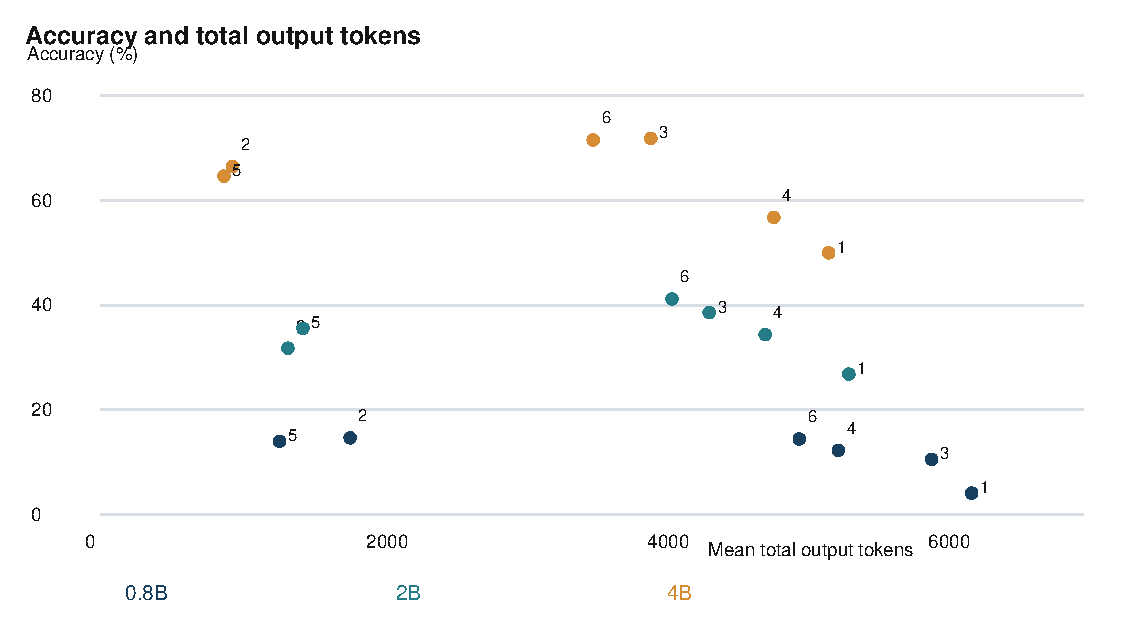
\includegraphics[width=\linewidth]{figures/tradeoff.pdf}\captionof{figure}{Each size has six points: 1 ON, 2 OFF, 3 selected limit, 4 LoRA alone, 5 LoRA + OFF, 6 LoRA + limit. All-attempt equal-problem summaries; overlapping points are retained. Lower tokens and higher accuracy are preferred.}\label{fig:tradeoff}\end{minipage}\end{center}

For 0.8B, OFF uses 1,781 mean output tokens compared with 6,206 for ON and 5,920 for the free selected limit. In the all-attempt view, the trained limit uses 4,979. These are problem-weighted lengths. The chart retains all responses, rather than describing only successful solutions.\par

The accuracy-token plot places each complete 0.8B configuration by its two measured averages. Moving left means shorter generated output and moving up means greater observed accuracy. A point's location does not include the expense of training or candidate selection. No time-per-token conversion is used to turn this plot into a latency estimate.\par

For 2B, OFF uses 1,337 mean output tokens compared with 5,331 for ON and 4,337 for the free selected limit. In the all-attempt view, the trained limit uses 4,072. These are problem-weighted lengths. The chart retains all responses, rather than describing only successful solutions.\par

The accuracy-token plot places each complete 2B configuration by its two measured averages. Moving left means shorter generated output and moving up means greater observed accuracy. A point's location does not include the expense of training or candidate selection. No time-per-token conversion is used to turn this plot into a latency estimate.\par

For 4B, OFF uses 943 mean output tokens compared with 5,188 for ON and 3,921 for the free selected limit. In the all-attempt view, the trained limit uses 3,511. These are problem-weighted lengths. The chart retains all responses, rather than describing only successful solutions.\par

The accuracy-token plot places each complete 4B configuration by its two measured averages. Moving left means shorter generated output and moving up means greater observed accuracy. A point's location does not include the expense of training or candidate selection. No time-per-token conversion is used to turn this plot into a latency estimate.\par

In the specific 4B first-attempt comparison, the free limit averages about 3,961 tokens and the trained limit about 3,511, a reduction of approximately 11.4\%. This reference token value differs from the all-attempt mean of about 3,921. The reduction statement uses the first-attempt reference consistently. An uncertain accuracy difference accompanies the measured length reduction.\par

\subsection*{4.8 Cap Rates and Historical Loop Evidence}\addcontentsline{toc}{subsection}{4.8 Cap Rates and Historical Loop Evidence}

\begin{center}\begin{minipage}{\linewidth}\centering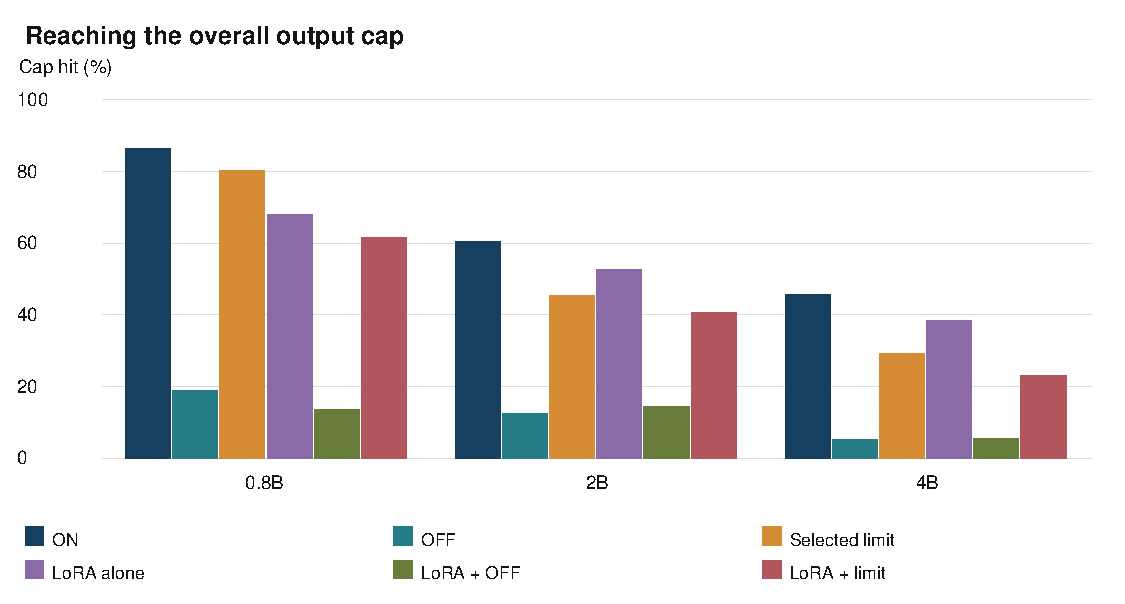
\includegraphics[width=\linewidth]{figures/caps.pdf}\captionof{figure}{Saved cap-hit rates across complete methods, using the combined problem-based summary. A cap hit is not a detected loop.}\label{fig:caps}\end{minipage}\end{center}

The full-coverage cap plot displays the saved hit-limit indicator. It reports whether the full response reached its output cap, not whether it met a repetition detector. OFF still has a cap rate because the answer itself can be long. A small thinking budget also does not guarantee a short complete response.\par

\begin{center}\begin{minipage}{\linewidth}\centering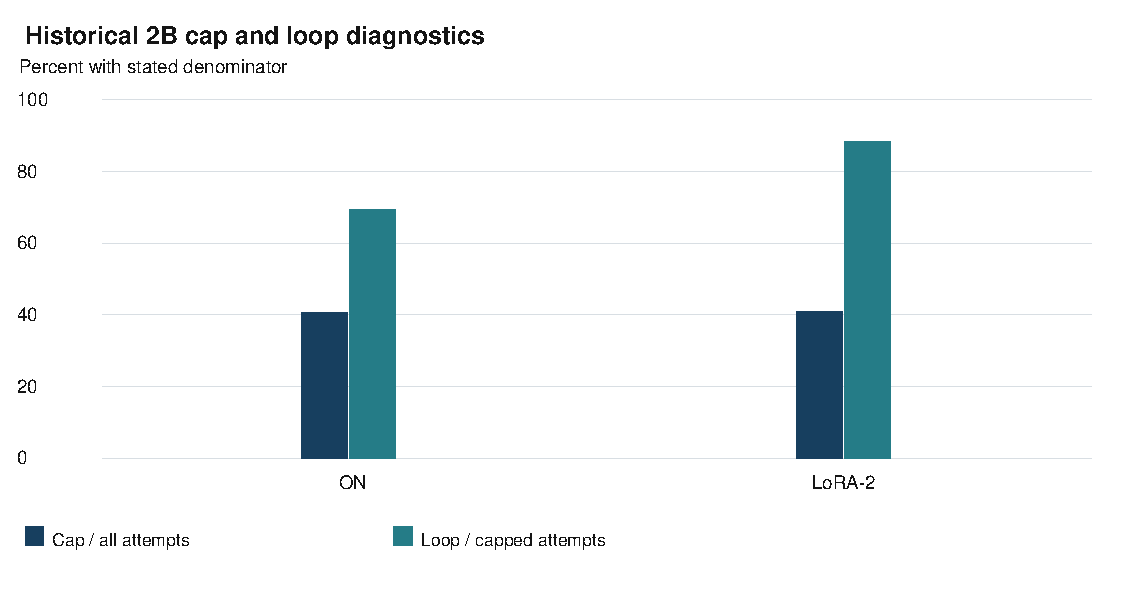
\includegraphics[width=\linewidth]{figures/loops.pdf}\captionof{figure}{Original 234-problem study with 468 attempts per method. Cap percentages use all attempts; loop percentages use capped attempts only. These are different denominators.}\label{fig:loops}\end{minipage}\end{center}

The historical 2B ON condition hits the cap on 190/468 attempts, or 40.6\%. Among those capped attempts, 69.5\% meet the saved loop rule. LoRA-2 hits the cap on 192/468 attempts, or 41.0\%, and 88.5\% of those capped attempts meet the rule. The denominator for a cap percentage is all attempts; the denominator for each loop percentage here is only capped attempts.\par

These loop findings refer to 234 original problems with two attempts per method. They are not computed for all 464 problems and should not be read as whole-study loop rates. The historical median thinking length of completed normal-thinking HumanEval+ answers is 672 tokens. Completion, length, and cap status describe related but distinct aspects of an answer.\par

\subsection*{4.9 Partial Sweeps and the Historical LoRA 2 Experiment}\addcontentsline{toc}{subsection}{4.9 Partial Sweeps and the Historical LoRA 2 Experiment}

\begin{center}\begin{minipage}{\linewidth}\centering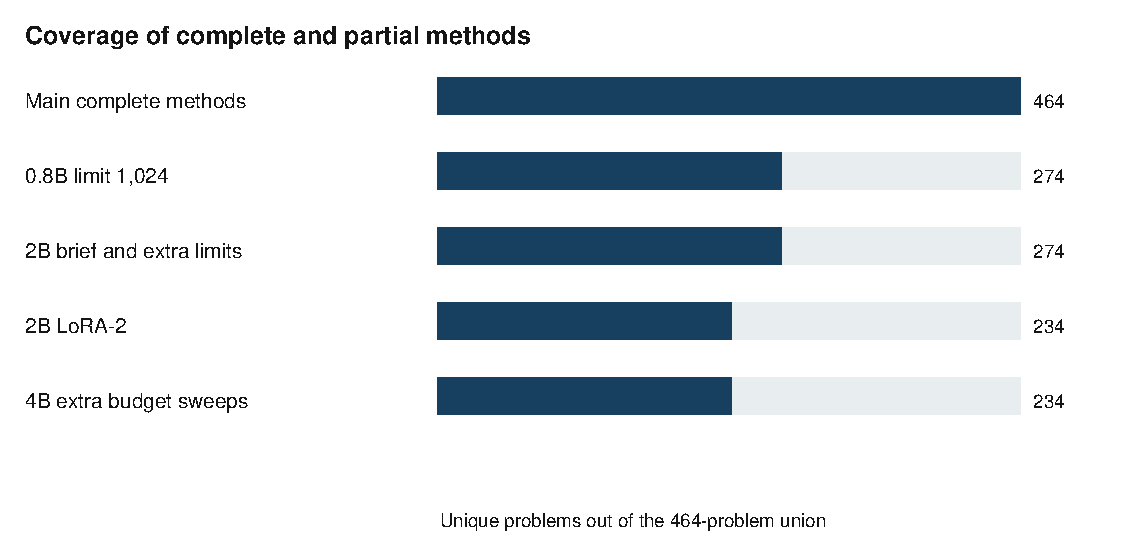
\includegraphics[width=\linewidth]{figures/coverage.pdf}\captionof{figure}{Coverage is a denominator, not a performance score. Partial sweeps cannot establish a result on unmeasured problems.}\label{fig:coverage}\end{minipage}\end{center}

\begingroup\singlespacing\small\setlength{\tabcolsep}{4pt}
\begin{longtable}{|p{1.130in}|p{1.130in}|p{1.130in}|p{1.130in}|p{1.130in}|}
\caption{Partial methods retained with actual coverage and all-attempt scoring}\label{tab:partial}\\
\hline
\textbf{Size} & \textbf{Method} & \textbf{Coverage} & \textbf{Attempts} & \textbf{Accuracy}\\\hline
\endfirsthead
\hline
\textbf{Size} & \textbf{Method} & \textbf{Coverage} & \textbf{Attempts} & \textbf{Accuracy}\\\hline
\endhead
0.8B & Limit 1024 & 274/464 & 274 & 11.3\%\\\hline
2B & Brief prompt & 274/464 & 548 & 6.4\%\\\hline
2B & Limit 2048 & 274/464 & 274 & 40.9\%\\\hline
2B & Limit 512 & 274/464 & 548 & 39.4\%\\\hline
2B & LoRA-2 & 234/464 & 468 & 45.1\%\\\hline
4B & Limit 1024 & 234/464 & 468 & 76.5\%\\\hline
4B & Limit 4096 & 234/464 & 468 & 76.7\%\\\hline
4B & Limit 512 & 234/464 & 468 & 75.4\%\\\hline
\end{longtable}
\endgroup

Some exploratory limits have high percentages on their covered subset. For example, the 4B limit sweep covers the original 234 problems, while the full-coverage selected limit covers the complete 464. A ranking that ignores those denominators would mix different task populations. The partial rows are included for completeness and are not promoted to full-set conclusions.\par

LoRA-2 covers 234 problems and has a 45.1\% equal-problem all-attempt accuracy in the combined record for that subset. It is a different add-on from LoRA-1. The original thinking-length ratio against normal thinking is 1.00 with an interval of 0.94 to 1.06. The historical study therefore did not observe the intended shortening under that analysis.\par

The brief-prompt result concerns one saved wording and its covered tasks. Saved examples indicate a conflict with the code-only instruction. The result does not measure every possible concise prompt. Similarly, a longer-output retry changes the generation conditions and remains a diagnostic outside the completed full-coverage comparisons.\par

\subsection*{4.10 Validation Results}\addcontentsline{toc}{subsection}{4.10 Validation Results}

\begingroup\singlespacing\small\setlength{\tabcolsep}{4pt}
\begin{longtable}{|p{1.997in}|p{1.997in}|p{1.997in}|}
\caption{Recorded evidence checks and their limits}\label{tab:validation}\\
\hline
\textbf{Check} & \textbf{Recorded outcome} & \textbf{Interpretation}\\\hline
\endfirsthead
\hline
\textbf{Check} & \textbf{Recorded outcome} & \textbf{Interpretation}\\\hline
\endhead
Unique test IDs & 464 & No duplicated ID in union\\\hline
Training-pool IDs checked & 280 & Exact overlap is zero\\\hline
Complete combinations & 6 x 464 answers & Same test IDs\\\hline
Notebook 24 answers & 2,320 & Five complete configurations\\\hline
Earlier 2B limit answers & 464 & Sixth configuration\\\hline
Grade / raw consistency & Checked in archive audit & No new code execution\\\hline
Bootstrap settings & 2,000; seed 3407 & Unadjusted problem intervals\\\hline
Semantic contamination & Not ruled out & ID checks are insufficient\\\hline
\end{longtable}
\endgroup

The combined dataset contains 464 unique test IDs. The training audit checks 280 saved training-pool IDs and reports no exact ID overlap. Every completed combination has 464 unique answers, 464 corresponding grades, and one attempt per ID according to the checked archive. The five Notebook 24 configurations contribute 2,320 answers, while the earlier 2B limit combination contributes 464.\par

The saved audit also checks recorded model settings, add-on hashes, raw/graded token agreement, expected IDs, and reference hashes. The document build validates the six complete pass counts against the checked summary values and records SHA-256 hashes of the evidence files. These checks establish consistency of the reporting inputs. They do not rerun the generated code or prove the absence of all possible benchmark contamination.\par

The PDF and Word formatting checks are separate from scientific validation. They confirm that captions, page numbering, and tables present the evidence coherently. A clean layout cannot strengthen an uncertain result, just as a correct calculation can still be misrepresented by an unlabeled chart. Both layers are therefore inspected before delivery.\par

\subsection*{4.11 Summary of Key Findings}\addcontentsline{toc}{subsection}{4.11 Summary of Key Findings}

The all-attempt free-control reference scores are 14.7\% for 0.8B OFF, 38.6\% for 2B limit 1,024, and 71.9\% for 4B limit 2,048. The completed trained limits reach 14.4\%, 41.2\%, and 71.6\%, respectively, with one answer per problem. These numbers use the attempt rules stated in their tables and are not a single unqualified ranking.\par

LoRA plus OFF does not consistently improve over OFF without LoRA. The 0.8B trained limit improves over its matching weak free limit, but does not establish a gain over the stronger OFF reference. The 2B and 4B trained limits have uncertain accuracy differences from their matching free limits. The 4B first-attempt comparison also records fewer total output tokens for the trained limit.\par

The historical diagnostics and partial sweeps remain informative at their own scope. They do not establish complete-set outcomes for untested budgets or a universal explanation for every failure. Chapter 5 interprets the main findings and explains what evidence a stronger follow-up would need.\par

\clearpage

\section*{Chapter 5: Discussion}\addcontentsline{toc}{section}{Chapter 5: Discussion}

\subsection*{5.1 Interpretation of the Main Results}\addcontentsline{toc}{subsection}{5.1 Interpretation of the Main Results}

The findings support a practical starting point: evaluate simple thinking controls before assuming that shortest-correct training is needed. In the all-attempt combined view, the best observed full-coverage free controls are OFF for 0.8B, limit 1,024 for 2B, and limit 2,048 for 4B. This is a statement about the measured collection and evaluated policies. It is not a claim that these settings are optimal for every prompt, code distribution, or deployment constraint.\par

The completed combinations add an important qualification. Training and thinking controls are not mutually exclusive alternatives. The same LoRA-1 add-on can be used with OFF or a limit. For 2B, the limit combination achieves the highest observed full-set accuracy at 191/464, or 41.2\%. Yet its lead over the matching free limit has an interval that includes zero. The report can identify the highest observed score without presenting the method as an established improvement over that reference.\par

For 4B, LoRA-1 plus limit 2,048 passes 332 problems, while the free-limit first attempt passes 330. A two-problem difference should be understood at its actual scale. The paired interval ranges from a possible disadvantage to a possible advantage. At the same time, the combination uses fewer output tokens than that first-attempt reference. This supports a measured token reduction with uncertain accuracy change, rather than a claim that accuracy has been proved equal.\par

For 0.8B, OFF without LoRA remains the highest observed full-coverage free score and is also slightly above both trained combinations. LoRA-1 plus limit improves over the weak free limit at the same budget, but that comparison is not the whole practical decision. A user considering additional training would also compare with the stronger OFF option. This illustrates why selecting only a favorable baseline can exaggerate an intervention's value.\par

\subsection*{5.2 Why a Matching Baseline Changes the Conclusion}\addcontentsline{toc}{subsection}{5.2 Why a Matching Baseline Changes the Conclusion}

Suppose the trained limited model is compared only with unrestricted thinking. Any gain could come from the learned add-on, from ending the thinking notes, or from their interaction. The comparison alone cannot separate these effects. A matching free limit makes the inference policy more comparable and asks whether training adds an observable benefit after the simple control is already present.\par

The completed 2B result demonstrates this distinction. LoRA plus limit is clearly above its historical unrestricted-thinking reference under the saved first-attempt analysis. Its much smaller difference from the free limit remains uncertain. The narrower conclusion is more useful for a deployment decision because the free limit is easier to try than collecting candidates and training an add-on.\par

The OFF combinations tell a similar story. LoRA plus OFF does not consistently beat OFF without LoRA across the three sizes. There is therefore no general finding that the add-on improves direct answering. The evidence does not establish that LoRA is inherently unsuitable for code generation; it evaluates these particular trained add-ons and their supervision.\par

Baseline choice is also connected to coverage. The higher percentage of a partially evaluated budget cannot replace a lower full-set baseline unless both are compared on the same relevant problems. A future study should choose its main comparison before viewing final test scores. In this retrospective report, the practical baselines are explicitly labeled as best observed among the full-coverage free settings.\par

\subsection*{5.3 A Possible Role for Repetition}\addcontentsline{toc}{subsection}{5.3 A Possible Role for Repetition}

The historical 2B diagnostic suggests that unfinished repeated thinking can consume a substantial part of the output budget. Under normal thinking, 190 of 468 attempts reached the cap, and 69.5\% of those capped attempts met the loop rule. Under LoRA-2, 192 attempts reached the cap, and 88.5\% of the capped attempts met that rule. These are measurements from the original 234 problems with two attempts each. They are not a 464-problem loop estimate.\par

A fixed thinking limit can force a transition out of the notes. This could leave enough output room for a program that would otherwise never appear. OFF avoids the explicit notes entirely. Both mechanisms are consistent with the observed improvements over unrestricted thinking. However, the study has not isolated the effect of repetition from every other change in response behavior.\par

Training only on completed correct examples may be poorly matched to a failure that involves not completing an answer. A successful target shows what a final response looks like, but it may not teach recovery once the model has entered a repeated pattern. This is a hypothesis about training coverage. A future intervention would need examples or controls that specifically target repetition and then measure whether that failure mode changes.\par

Cap hits must still be interpreted cautiously. A capped answer can contain executable code, and an uncapped answer can be wrong. Likewise, not every long response is redundant. The thesis therefore reports correctness, output length, and cap behavior separately. Combining them into a single label such as overthinking failure would lose useful distinctions.\par

\subsection*{5.4 What the Training Data Can Explain}\addcontentsline{toc}{subsection}{5.4 What the Training Data Can Explain}

The historical LoRA-2 data show that starting with 280 problems did not provide 280 short correct training targets. Only 157 examples were retained. Moreover, the contest examples remained much longer than the function examples, with little selected-length advantage over average correct candidates. This limits the strength of the concise supervision available for contest tasks.\par

The natural interpretation is that a selection procedure can only choose among the candidate behaviors it sees. If the model has no short passing solution for a task, selecting the shortest passing candidate may still yield a long trace. Adding more problems to the starting pool is therefore different from adding more examples of the desired behavior. The pool size, success rate, and retained-length distribution all matter.\par

LoRA-2's falling loss shows improved fit to its selected examples. The original held-out thinking-length ratio remains about 1.00, with an interval from 0.94 to 1.06. These observations can coexist. Optimization can succeed on its training objective without delivering the hoped-for generalization. This is a familiar distinction in empirical learning systems, and it should not be hidden by describing the training run alone as successful compression.\par

The LoRA-1 comparisons add another limit. The sizes do not share exactly the same retained training examples or identical response dynamics. The higher performance of 4B is therefore not a controlled estimate of the benefit of parameter count alone. The systems should be compared as tested configurations, with a future standardized experiment needed to isolate model scale.\par

\subsection*{5.5 Benchmark and Difficulty Differences}\addcontentsline{toc}{subsection}{5.5 Benchmark and Difficulty Differences}

HumanEval+ function completion and LiveCodeBench contest tasks differ in interface, required solution structure, and problem distribution. The result tables show these groups separately because an overall score can hide severe weakness on medium contest tasks. A configuration that succeeds on many functions may still be unreliable when it must parse input, implement a longer algorithm, and print exact output.\par

The group sizes also shape the combined result. HumanEval+ contributes 164 of 464 problems, LiveCodeBench easy contributes 166, and medium contributes 134. Equal problem weighting means these groups contribute in proportion to those counts. The report does not assign equal weight to each benchmark category independently. Changing to equal category weights would define another statistic and should be labeled as such.\par

Group breakdowns are descriptive, not independent replications. The same 464 problems are being reorganized into subsets. A striking subgroup difference may suggest a follow-up question, but multiple subgroup comparisons also create opportunities for chance patterns. The thesis does not select a favorable subgroup and treat its result as the primary study conclusion.\par

The labels easy and medium do not imply that the 0.8B model finds those problems easy. Difficulty categories come from the source benchmark. A small model can fail almost every task in a category that is relatively accessible to a human contestant. The reader should interpret difficulty alongside the measured score rather than as a prediction of model success.\par

\subsection*{5.6 Accuracy, Tokens, and Practical Choice}\addcontentsline{toc}{subsection}{5.6 Accuracy, Tokens, and Practical Choice}

Accuracy and output tokens express different priorities. If a user needs the highest observed passing rate for a fixed model, a limit can be attractive. If the user needs short output, OFF may be a better starting point. A scatter plot helps show the tradeoff, but it does not determine a universal winner because the acceptable cost of an error depends on the application.\par

\begin{center}\begin{minipage}{\linewidth}\centering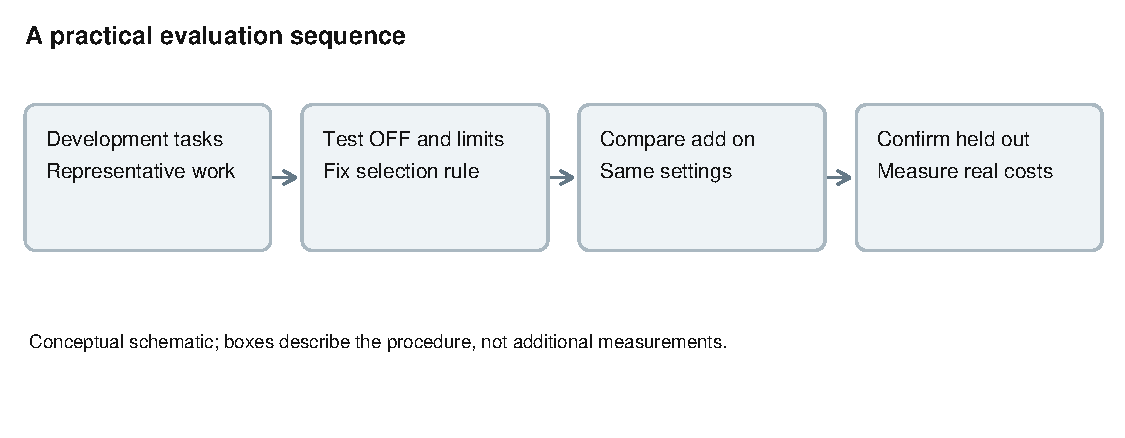
\includegraphics[width=\linewidth]{figures/decision.pdf}\captionof{figure}{Suggested follow-up workflow. It is a recommendation, not an additional completed evaluation.}\label{fig:decision}\end{minipage}\end{center}

For 4B, the trained limit combination's approximately 11.4\% reduction in total output tokens relative to the historical first-attempt free limit is relevant. It indicates fewer generated tokens in this comparison. It does not prove a corresponding 11.4\% latency or cost reduction. Time per token, batch utilization, model loading, and training amortization can all affect an operational decision.\par

For 2B, training plus a limit yields a higher point estimate than the free limit, but the remaining uncertainty matters. A small apparent advantage may be valuable in one setting and insufficient to justify training in another. Before deployment, the user should evaluate a separate development collection representative of the intended workload and then confirm the chosen policy on held-out problems.\par

For 0.8B, the simple OFF policy offers a strong practical reference within this study. Its observed accuracy is low in absolute terms, which also matters. A method can be the best measured option for a weak model and still be unsuitable for unsupervised use. The thesis recommends a starting policy for testing; it does not claim that the resulting programs require no review.\par

\subsection*{5.7 Comparison with Prior Work}\addcontentsline{toc}{subsection}{5.7 Comparison with Prior Work}

The results are compatible with a broad lesson from the reviewed literature: useful reasoning efficiency depends on the model, task, and intervention. Concise self-training is a motivated approach, and explicit thinking can also be unnecessary under some conditions. Our evidence adds a specific case in which strong free controls change how the trained method should be interpreted.\par

This study is not a numerical reproduction of any cited compression paper. The base models, parameter scales, datasets, retained examples, inference rules, and outcome definitions differ. It would be misleading to compare a reduction percentage from another paper directly with this thesis's total-token change and declare one approach superior. The measures may concern different portions of the output and different test populations.\par

The most useful comparison is conceptual. Prior methods show why successful concise supervision is worth testing. The present results show why a matching free control and an explicit attempt rule belong in that test. This combination improves the quality of the empirical question even when a method does not achieve the hoped-for outcome.\par

\subsection*{5.8 Threats to Validity}\addcontentsline{toc}{subsection}{5.8 Threats to Validity}

Internal validity concerns whether the measured difference can be attributed to the intervention. Historical package changes, differing batch layouts, stopping behavior, and unequal attempt counts limit that attribution. Matching problem IDs and first attempts improves clarity, but does not create a contemporaneous randomized experiment after the fact. A future replication should standardize the environment and execution order.\par

Construct validity concerns whether the metrics represent the intended concept. Passing used tests is a practical measure of functional correctness, but not a formal proof. Token count measures response length, but not directly elapsed time or energy. A cap hit indicates a stopping event, but not necessarily a loop. The report keeps these constructs separate.\par

External validity concerns transfer beyond the measured setting. The study covers one model family, Python code, 464 problems, and no hard contest tasks. It does not establish results for larger instruction models, different languages, interactive debugging, or real repositories. The selected task mixture also influences the combined score.\par

Statistical conclusion validity concerns uncertainty and selection. The intervals are unadjusted, many comparisons are possible, and the combined view was selected after the results. The displayed precision reflects arithmetic, not freedom from bias. An inconclusive interval is not evidence of equivalence, and a positive interval is not a guarantee on a new population.\par

Training/test separation is checked at the ID level, with historical text exclusions preserved. Semantic similarity and pretraining exposure remain possible. The absence of a matching ID should not be described as contamination-free evaluation. Benchmark release timing can reduce one concern without proving what the base model encountered during its creation.\par

\subsection*{5.9 Reporting Lessons and Implications}\addcontentsline{toc}{subsection}{5.9 Reporting Lessons and Implications}

The study illustrates why clear labels are part of experimental quality. The 4B free limit can correctly appear as 71.9\% in one table and 71.1\% in another when the attempt rules differ. Without an explanation, the reader could interpret that as an error or select whichever figure helps a preferred story. The same principle applies to the all-attempt and first-attempt LoRA values for 2B.\par

The completed-control results also show the value of reporting a negative or uncertain answer directly. A study does not need to demonstrate a new winner to be useful. Establishing that a trained add-on has not shown a reliable accuracy gain over a simpler setting can guide the next use of research time. It narrows the intervention that needs testing rather than encouraging more of the same experiments without a clear question.\par

For researchers, the next design should make the matched free control part of the original protocol. For practitioners, the first step should be a low-cost evaluation of OFF and a few development-chosen limits. For readers, the main discipline is to ask what changed between the compared rows and which problems and attempts support the percentages.\par

\subsection*{5.10 Chapter Summary}\addcontentsline{toc}{subsection}{5.10 Chapter Summary}

Simple controls explain much of the practical improvement over unrestricted thinking in the saved study. The completed combinations are informative, but the 2B and 4B accuracy gains over their matching free limits remain uncertain. Historical repetition and training-data analyses suggest plausible mechanisms without proving them. The conclusion therefore emphasizes measured tradeoffs, explicit uncertainty, and a more controlled next experiment.\par

\clearpage

\section*{Chapter 6: Conclusion and Future Work}\addcontentsline{toc}{section}{Chapter 6: Conclusion and Future Work}

\subsection*{6.1 Summary of the Study}\addcontentsline{toc}{subsection}{6.1 Summary of the Study}

This thesis examined shortest-correct LoRA training and thinking controls for Qwen3.5-0.8B, 2B, and 4B on a combined collection of 464 coding problems. The test set contains 164 HumanEval+ functions and 300 LiveCodeBench tasks, including 166 easy and 134 medium problems. The report uses saved outputs and grades, with no new model training or generation for the document build.\par

The study compares inference controls that require no additional training with saved trained add-ons. It also evaluates all six planned combinations of LoRA-1 with OFF or a selected thinking limit. The central comparison is whether the trained system improves over a matching free policy, rather than merely over unrestricted thinking. Accuracy and output tokens are reported together, with coverage and attempt rules kept visible.\par

\subsection*{6.2 Answers to the Research Questions}\addcontentsline{toc}{subsection}{6.2 Answers to the Research Questions}

For RQ1, the best observed full-coverage free controls differ by model size. In the equal-problem all-attempt summary, OFF reaches 14.7\% for 0.8B, limit 1,024 reaches 38.6\% for 2B, and limit 2,048 reaches 71.9\% for 4B. These are the best among the measured full-coverage free settings, not established globally optimal budgets. OFF generates the fewest output tokens among the main free controls at each size.\par

For RQ2, the selected free controls score above LoRA-1 alone in the all-attempt paired summaries. The 0.8B advantage remains uncertain, while the saved 2B and 4B intervals favor the selected free controls. This supports testing simple controls before investing in this training procedure. It does not show that every LoRA design or every possible concise training set is ineffective.\par

For RQ3, all six LoRA combinations are complete with one answer per problem. The OFF and limit pass totals are 65 and 67 for 0.8B, 165 and 191 for 2B, and 300 and 332 for 4B. The 2B trained limit has the highest observed full-set point estimate for that size, at 41.2\%. Its gain over the matching free limit remains uncertain. The 4B trained limit reaches 71.6\% and similarly has no established accuracy advantage over the free-limit first attempt.\par

For RQ4, the benchmark breakdowns show why the task mixture must remain visible. HumanEval+ and contest groups have different observed outcomes, and medium contest tasks remain particularly challenging for the smallest model. The combined score is a weighted summary of this specific collection. It cannot replace group-level inspection when the intended application resembles only one part of the benchmark.\par

For RQ5, the historical loop and training analyses provide possible explanations for long output and limited transfer. They retain their original 234-problem scope. LoRA-2 did not show the desired shortening in that experiment, and many capped outputs satisfied the saved loop rule. These observations motivate a targeted recovery intervention, but they do not establish a general causal account for every later result.\par

\subsection*{6.3 Main Conclusions}\addcontentsline{toc}{subsection}{6.3 Main Conclusions}

The clearest conclusion is methodological: compare a trained reasoning method with a strong, matching inference control. A gain over unrestricted thinking can be real while providing little evidence that the training component is needed. In this study, OFF and fixed thinking limits are essential references for understanding the trained combinations.\par

The practical conclusion is conditional. Begin with the observed free policy for the model size and evaluate it on representative development tasks. Consider a trained combination if its measured accuracy and token tradeoff justifies the added work in that application. In particular, the 4B limit combination provides a measured reduction in output tokens with an uncertain accuracy change, rather than demonstrated equivalence or a guaranteed improvement.\par

The scientific conclusion is bounded by the study design. The combined analysis is retrospective, uses historical references, and covers one model family and a limited code collection. The intervals are unadjusted, and the LiveCodeBench grader uses up to 20 tests per problem. These limitations remain part of the conclusion rather than being confined to a footnote.\par

\subsection*{6.4 Recommendations for Future Work}\addcontentsline{toc}{subsection}{6.4 Recommendations for Future Work}

The first follow-up should use a single saved software environment and a prospectively fixed evaluation protocol. It should compare the base model and the same add-on under ON, OFF, and a development-chosen limit. Test problems should remain untouched until settings are fixed. Multiple generation and training seeds would help distinguish stable policy effects from sampling and optimization variation.\par

The second follow-up should change the training supervision in a specific way. One candidate is to train on correct answers generated under a thinking limit, rather than only selecting from unrestricted candidates. Another is to include recovery examples that demonstrate leaving a repeated reasoning pattern and completing code. These are proposed interventions, not completed experiments in the present report.\par

The third follow-up should separate answer-format failure, incomplete generation, detected repetition, runtime failure, and incorrect computation. This would require a documented classification procedure applied to saved outputs. Such an analysis could test whether a limit mainly improves answer completion or also changes the quality of algorithms that reach the final answer.\par

The fourth follow-up should measure end-to-end resources. It should record wall-clock latency, accelerator use, batch behavior, and the up-front expense of candidate generation and training. Token counts should remain available as a portable metric, but actual measurements are needed before making claims about cost savings or deployment speed.\par

The fifth follow-up should broaden validation with a separate benchmark collection, hard contest problems, and another model family. It should also conduct a semantic training/test similarity review rather than rely only on IDs. These extensions would test external validity while preserving the clear baseline and reporting rules established here.\par

\subsection*{6.5 Closing Statement}\addcontentsline{toc}{subsection}{6.5 Closing Statement}

Small reasoning models should be judged by the code they successfully produce and the resources they actually use. The saved study shows that ending or disabling explicit thinking can be a strong practical intervention. Shortest-correct training remains a testable idea, but its benefit must be demonstrated beyond the simple controls already available. Clear denominators, matched comparisons, and honest uncertainty make that conclusion useful and reproducible.\par

\clearpage

\begin{thebibliography}{99}\addcontentsline{toc}{section}{References}

\bibitem{survey} Y. Sui et al., ``Stop Overthinking: A Survey on Efficient Reasoning for Large Language Models,'' 2025. [Online]. Available: \url{https://arxiv.org/abs/2503.16419}. Accessed: Oct. 20, 2026.

\bibitem{q08} Qwen Team, ``Qwen3.5-0.8B model card,'' 2026. [Online]. Available: \url{https://huggingface.co/Qwen/Qwen3.5-0.8B}. Accessed: Oct. 20, 2026.

\bibitem{q2} Qwen Team, ``Qwen3.5-2B model card,'' 2026. [Online]. Available: \url{https://huggingface.co/Qwen/Qwen3.5-2B}. Accessed: Oct. 20, 2026.

\bibitem{q4} Qwen Team, ``Qwen3.5-4B model card,'' 2026. [Online]. Available: \url{https://huggingface.co/Qwen/Qwen3.5-4B}. Accessed: Oct. 20, 2026.

\bibitem{lora} E. J. Hu et al., ``LoRA: Low-Rank Adaptation of Large Language Models,'' 2021. [Online]. Available: \url{https://arxiv.org/abs/2106.09685}. Accessed: Oct. 20, 2026.

\bibitem{selftrain} T. Munkhbat et al., ``Self-Training Elicits Concise Reasoning in Large Language Models,'' 2025. [Online]. Available: \url{https://arxiv.org/abs/2502.20122}. Accessed: Oct. 20, 2026.

\bibitem{seer} K. Huang et al., ``SEER: Self-Enhancing Chain-of-Thought Compression for Reasoning Models,'' 2026. [Online]. Available: \url{https://arxiv.org/abs/2509.14093}. Accessed: Oct. 20, 2026.

\bibitem{asap} W. Zeng et al., ``Pruning the Unsurprising: Efficient LLM Reasoning via First-Token Surprisal,'' 2026. [Online]. Available: \url{https://arxiv.org/abs/2508.05988}. Accessed: Oct. 20, 2026.

\bibitem{nothink} W. Ma et al., ``Reasoning Models Can Be Effective Without Thinking,'' 2025. [Online]. Available: \url{https://arxiv.org/abs/2504.09858}. Accessed: Oct. 20, 2026.

\bibitem{s1} N. Muennighoff et al., ``s1: Simple test-time scaling,'' 2025. [Online]. Available: \url{https://arxiv.org/abs/2501.19393}. Accessed: Oct. 20, 2026.

\bibitem{evalplus} J. Liu, C. S. Xia, Y. Wang, and L. Zhang, ``Is Your Code Generated by ChatGPT Really Correct? Rigorous Evaluation of Large Language Models for Code Generation,'' 2023. [Online]. Available: \url{https://arxiv.org/abs/2305.01210}. Accessed: Oct. 20, 2026.

\bibitem{lcb} N. Jain et al., ``LiveCodeBench: Holistic and Contamination Free Evaluation of Large Language Models for Code,'' 2024. [Online]. Available: \url{https://arxiv.org/abs/2403.07974}. Accessed: Oct. 20, 2026.

\bibitem{mbpp} J. Austin et al., ``Program Synthesis with Large Language Models,'' 2021. [Online]. Available: \url{https://arxiv.org/abs/2108.07732}. Accessed: Oct. 20, 2026.

\end{thebibliography}

\clearpage\section*{Appendix A: Evidence and Supplementary Data}\addcontentsline{toc}{section}{Appendix A: Evidence and Supplementary Data}

The companion source/evidence folder preserves checked result summaries and all 464 test IDs. The evidence manifest records SHA-256 hashes. The original repository retains raw outputs, grades, and environment files. No training problem is included in the main test total.

\section*{Appendix B: Reproduction Procedure}

Compile main.tex with pdfLaTeX at least twice. Compile conference.tex separately. The bibliography is embedded for portable compilation; references.bib is supplied for reuse. The Python builder uses the original repository layout and performs no model generation. The Word document supports field updates and Google Docs import.

\section*{Appendix C: Further Checks and Authorship Details}

See originality-review.md for the scope and limits of textual overlap checks. Personal and institutional fields are placeholders. Signatures remain blank. A commercial plagiarism certificate has not been produced.

\end{document}